% Citadel-Rx, EXTENDED version (19 pages, every result and proof in full); the journal version is ../main.tex.
% Compile here: pdflatex main_extended (twice). Figures: ../../docs/figures.
% Every result number is a macro \val{key} defined in numbers.tex, and every result table body is
% a file in tables/; both are written by scripts/revision_numbers.py from the run records in
% results/. The submitted version is main_submitted.tex.
\documentclass[journal]{IEEEtran}
\usepackage{amsmath,amssymb,amsthm,bm}
\usepackage{graphicx}
\usepackage{booktabs,multirow,array,makecell}
\renewcommand{\theadfont}{\scriptsize}
\usepackage{xcolor}
\usepackage{algorithm}
\usepackage{algpseudocode}
\usepackage{tikz}
\usetikzlibrary{arrows.meta,positioning,fit,backgrounds}
\usepackage[hidelinks]{hyperref}
\usepackage{cite}
\usepackage{url}
\graphicspath{{../../docs/figures/}}

\newtheorem{theorem}{Theorem}
\newtheorem{lemma}{Lemma}
\newtheorem{proposition}{Proposition}
\theoremstyle{remark}
\newtheorem{remark}{Remark}
\newcommand{\norm}[1]{\left\lVert #1 \right\rVert}
\newcolumntype{L}[1]{>{\raggedright\arraybackslash}p{#1}}
\setlength{\tabcolsep}{3pt}
\setlength{\textfloatsep}{8pt plus 2pt minus 2pt}\setlength{\floatsep}{6pt plus 2pt minus 2pt}\setlength{\intextsep}{6pt plus 2pt minus 2pt}\setlength{\dbltextfloatsep}{8pt plus 2pt minus 2pt}\setlength{\dblfloatsep}{6pt plus 2pt minus 2pt}
% \val{key}: a number computed by scripts/revision_numbers.py; a missing key prints in red
\makeatletter
\newcommand{\val}[1]{\@ifundefined{val@#1}{\textcolor{red}{[\texttt{\detokenize{#1}}?]}}{\@nameuse{val@#1}}}
\newcommand{\tab}[1]{\@@input ../tables/#1.tex }   % table body written by scripts/revision_numbers.py
\newcommand{\ifval}[3]{\@ifundefined{val@#1}{#3}{#2}}   % text that needs a result not computed yet
\makeatother
\InputIfFileExists{../numbers}{}{}
\tikzset{
  blk/.style={draw=black!70,rounded corners=1pt,align=center,font=\scriptsize,inner sep=3pt,minimum height=6mm,fill=white},
  mem/.style={blk,fill=black!8}, gat/.style={blk,fill=black!18},
  grp/.style={draw=black!50,dashed,rounded corners=2pt,inner sep=2.5mm},
  arr/.style={-{Latex[length=1.5mm]},thin,draw=black!80}, darr/.style={-{Latex[length=1.5mm]},thin,dashed,draw=black!80},
  lbl/.style={font=\tiny,fill=white,inner sep=1pt}}

\begin{document}

\title{Memory Is the Defence: Physics-Gated Continuum-Memory Receivers for Poisoning-Resilient Test-Time Learning}

\author{Abraheem~Rashid%
\thanks{A. Rashid is with the Department of Computer Science, Brunel University London, London, U.K. (e-mail: 2546393@brunel.ac.uk).}%
\thanks{Code, configuration files, every run record, the statistics and the scripts that regenerate every table, figure and number of this paper are available at \url{https://github.com/abraheemrashid99-sys/Citradel-Rx}; three commands re-run the two campaigns and one (\texttt{make paper}) rebuilds every number, table and figure and the paper (Section~\ref{sec:setup}).}}

\markboth{IEEE Transactions on Wireless Communications}{Rashid: Memory Is the Defence}
\maketitle

\begin{abstract}
A test-time neural receiver trains on pilots an adversary can write to; this paper argues it should consolidate into persistent memory only what a label-free physical check verifies against that memory.
Citadel-Rx applies this to DeepSIC: a fast level fitted per block feeds two slow levels through a
gated average whose clip bounds how far any attacker moves the slowest level per consolidation.
With a single memory, a cyclic redundancy check test with rollback fails, as do Citadel-Rx's gates:
their only reference, linear minimum mean-square error (LMMSE) detection on the poisoned pilots,
degrades too. On ten held-out seeds of the stationary benchmark channel, white-box poisoning (A1) at
0\,dB signal-to-interference ratio raises the symbol error rate (SER) of Citadel-Rx by
\val{p1.citadel.wb0.excess}, against \val{p1.online_deepsic.wb0.excess} for tuned online DeepSIC and
\val{p1.ml.wb0.excess} for maximum-likelihood detection (better on clean blocks); the gates reject
\val{p1.citadel.wb0.rej} of poisoned and \val{p1.citadel.wb0.frej} of clean blocks,
\val{deny.citadel.frej} after a legitimate channel redraw (SER \val{deny.citadel.after}, online DeepSIC
\val{deny.onlinedeepsic.after}). Full-budget adapted attacks, rejected on nearly every block, gave an
excess not distinguishable from plain A1 with four or five seeds; one testing candidates on an exact
receiver copy passes the gates only at about \val{orc.acc.scale} of its budget, leaving almost no
excess afterwards. The worst attack found without a channel change, A4 (pilots and data, 20 gradient
steps), gives \val{b2.a4pgd20.excess}; poisoning during one also raises the excess. Citadel-Rx fails
at 16-QAM and in a coded 5G link over 3GPP urban-micro channels, where its network is weaker than
LMMSE on clean blocks.
\end{abstract}

\begin{IEEEkeywords}
Deep receivers, test-time learning, adversarial pilot poisoning, continual learning, physics-informed gating, MIMO detection, physical-layer security.
\end{IEEEkeywords}

\section{Introduction}
\IEEEPARstart{D}{eep} receivers replace or augment the model-based blocks of a receiver
with neural networks trained on data \cite{oshea2017,honkala2021,samuel2019,shlezinger2023}.
Since a network trained in simulation meets a different channel in the field, the strongest deep receivers adapt at test time: online DeepSIC \cite{shlezinger2021} re-trains its per-user networks from
block to block, and Meta-DeepSIC \cite{raviv2023} meta-learns an
initialisation from past blocks so that the per-block fit converges faster. In \cite{raviv2023} the
training data of a block are its decoded codewords, re-encoded and used as labels when decoding
succeeds, and no new pilots are sent; in the pilot-trained form attacked in \cite{wu2024} and
studied here, the adaptation data are the only labelled symbols the receiver sees: a few hundred
pilot bits per user per block.

An adversary within range of the base station can add a perturbation to the received pilot part
of a block. Wu \emph{et al.} \cite{wu2024} showed that a perturbation of the pilots, crafted on a surrogate
receiver without knowledge of the target, transfers to online DeepSIC, to Meta-DeepSIC and to two
other online detectors and impairs their adaptation. In the runs reported here
(Section~\ref{sec:headline}), a white-box perturbation shaped through an unrolled copy of the
receiver's adaptation step, at a signal-to-interference ratio of $0$\,dB, raises the symbol error
rate (SER) of online DeepSIC by \val{p1.online_deepsic.wb0.excess} over its clean run, and
Meta-DeepSIC, which keeps the poisoned pilots in its support set, still carries an excess after the
attack stops. The receiver cannot verify its adaptation data, because the pilots are the labels. It can verify physical consistency: whether its decisions fit a linear channel model, whether the cyclic redundancy check (CRC) of the decoded data passes, and whether the estimated channel changed as a fading channel does from one block to the next. The harm of poisoning lies less in the attacked block than in what the receiver keeps.

This paper argues for one principle: \emph{a test-time receiver resists pilot poisoning when it
consolidates into persistent memory only what an independent, label-free physical check
verifies, and when that check judges every update against the protected memory.} It is a design condition supported by an ablation, not a guarantee: a receiver that meets it still fails where its network is weaker than the linear minimum mean-square error (LMMSE) detector on clean blocks, where the attacker also degrades the references through the data, and during a legitimate channel change (Section~\ref{sec:discussion}). The two parts
depend on each other. The simplest receiver with a check and a memory, online DeepSIC with a CRC test and rollback to its last accepted weights, fails. Its only reference is LMMSE on the same poisoned pilots, which the attack degrades together with the update. The first poisoned update therefore passes the relative test and becomes the state the receiver rolls back to, and every later update starts from it (Section~\ref{sec:c1}). The receiver proposed here, Citadel-Rx, fails in the same way when it is given its gates but only a single memory (Section~\ref{sec:ablate}). Citadel-Rx keeps memory at three rates, a fast level that
fits every block and two slow levels that change only through a gated, clipped average of the
faster states, and its gates compare the fast level with the better of LMMSE on the pilots of the
block and a detector built on the slow memory (the anchor detector), which those pilots do not reach. Multi-rate memory is one realisation of the principle;
the ablation shows which of its parts are necessary.

\begin{table}[t]
\centering\caption{Positioning. Attack surface: what the adversary writes to. Online DeepSIC and Meta-DeepSIC are listed in the pilot-trained form attacked in \cite{wu2024}.}\label{tab:pos}
\scriptsize
\begin{tabular}{@{}L{23mm}L{12mm}L{15mm}L{29mm}@{}}
\toprule
Class & Adapts & Memory & Attack surface / defence\\
\midrule
LMMSE & no & -- & pilot estimate / --\\
Pilot-spoofing detection \cite{kapetanovic2013,tugnait2015} & no & -- & pilots / detection only\\
Online DeepSIC \cite{shlezinger2021} & every block & last block & pilots / --\\
Meta-DeepSIC \cite{raviv2023} & every block & pilot buffer & pilots, persistent / --\\
Code-verified online training \cite{viterbinet2020,schibisch2018} & on decoded data & last block & labels / code check, no persistent gate\\
CRC-Rollback (Section~\ref{sec:c1}) & every block & last accepted & pilots / CRC gate, rollback\\
Filtering and restoring TTA \cite{eata2022,cotta2022,sar2023,rotta2023} & every batch & weights, anchor & batch / entropy filter, restore\\
Robust TTA \cite{medbn,wu2023tta} & every batch & batch statistics & batch / robust statistics\\
Anchored fine-tuning \cite{l2sp2018,ewc2017,meanteacher2017} & every step & prior or averaged weights & data / pull to a prior or a teacher\\
Nested, continuum memory \cite{behrouz2025nested,behrouz2025titans} & every token & one or several rates & input / --\\
Citadel-Rx (this paper) & every block & three rates, gated & pilots / physics gates, protected fallback, bounded retention\\
\bottomrule
\end{tabular}
\end{table}

Table~\ref{tab:pos} places the design among the work it draws on. Pilot spoofing is an
established physical-layer threat \cite{zhou2012pilot,kapetanovic2015}, with detectors that
flag it \cite{kapetanovic2013,tugnait2015}, but that work has no learning receiver to protect. Decision-directed
training on decoded data verified by the code is the closest precedent for using the code check
to decide what a receiver learns from \cite{viterbinet2020,schibisch2018}, and Meta-DeepSIC was proposed with it \cite{raviv2023}; it verifies labels, not what enters a
persistent memory. In deep receivers, drift detection decides when, and which module, to re-train \cite{uzlaner2024}, and Bayesian tracking replaces the multi-step fit of a block by a single-step update of a posterior over the weights \cite{gusakov2025}; both address channel variation, not an adversary. In vision, test-time adaptation (TTA) filters, anchors or restores what enters the
adapted weights \cite{eata2022,cotta2022,sar2023,rotta2023,persistent2024}, anchors fine-tuning to a
prior, as transfer and continual learning do \cite{l2sp2018,ewc2017}, or averages a teacher, as semi-supervised learning does \cite{meanteacher2017}. It has its own
poisoning problem \cite{wu2023tta,cong2024}, smaller when the attacker sees neither the online weights nor other users' samples \cite{su2025}, with robust-statistics defences \cite{medbn}; a periodic reset to the pre-trained weights matches or betters continual adaptation over long streams \cite{rdumb2023}. These methods
work without a physical check such as a code; the EATA- and CoTTA-style, anchored, teacher and median forms are compared below in receiver form. Byzantine-robust aggregation
\cite{blanchard2017} needs many gradient vectors per step, certified defences against data
poisoning \cite{steinhardt2017} bound the loss of a convex learner, and a theory of continual learning under poisoning \cite{hu2026} treats regularisation-based learners over a sequence of tasks, with a defence that flags a task by comparing consecutive updates; here the learner is a network
that sees one correlated block at a time. Nested learning \cite{behrouz2025nested} and Titans
\cite{behrouz2025titans} learn memory at test time, the first at several update rates and the second in one
long-term module written in proportion to a surprise measure; neither has a test that can refuse a write, and gated fast-to-slow consolidation echoes complementary learning systems
\cite{mcclelland1995,kumaran2016}. Adversarial examples against deep physical-layer models
\cite{sadeghi2019,sadeghi2019ae}, over-the-air poisoning of a wireless learner that re-trains on sensed data \cite{sagduyu2021}, and the methodology of attacks adapted to a defence
\cite{athalye2018obfuscated,carlini2019,tramer2020} shape the evaluation. To the author's knowledge, no published deep receiver combines multi-rate memory, physics-gated consolidation and a retention bound.

The contributions are as follows.
\begin{enumerate}
\item \textbf{The principle and a receiver that realises it} (Section~\ref{sec:citadel}): gated,
clipped consolidation into two slow levels, a fallback that detects a rejected block with the
slow memory, and per-sub-block CRC selection among the fast, slow and LMMSE decisions; the
ablation identifies a slow level (the excess SER is \val{ab.K1.excess} without one, \val{ab.K2.excess} with one and \val{ab.complete.excess} with two), the fallback and a decision-level gate
as necessary, and
attributes most of the clean-SER gain to the CRC selection.
\item \textbf{Retention bounds for the algorithm as implemented} (Section~\ref{sec:theory}): a
design bound, with no measured quantity, on the paired displacement of the slowest level under
any attacker, and a structural bound for unequal gate verdicts computed from the paired
trajectories. An error in the consolidation rule of an earlier version of this receiver (the first version below), which broke the convexity the
bounds rely on, is corrected.
\item \textbf{Relative physics gates with a CRC design rule} (Section~\ref{sec:gates}): three
label-free ratio tests and a design rule for the CRC threshold. Two tests compare the model residual and the CRC pass fraction of the fast level with those of the better of LMMSE and the anchor detector on the same block; the third compares the channel innovation with its running level. The rule sets the CRC threshold by a target excess symbol-error probability over that reference. The evaluated receiver uses the relative slack with a floor of $2\cdot10^{-3}$, which calibration chose over a slack derived from the pass-fraction statistics that follows the block length (Table~\ref{tab:cal}); the derived rule is therefore an analysis, not what was evaluated.
\item \textbf{An evaluation with tuned baselines and attacks adapted to the defence} (Sections~\ref{sec:setup}--\ref{sec:results}).
The baselines, among them CRC-Rollback and anchored, decision-directed, EATA-style and CoTTA-style
receivers, use the optimiser setting tuned for online DeepSIC and their own settings at default
values, except the L2-SP weight, which is swept. The attacks are built against the defence (soft gates, deep unrolling, restarts, expectation over noise, joint pilot and data
poisoning of the references, denial of adaptation, a slow small-budget attack optimised to be
accepted, a grey-box surrogate, a query attacker that did not converge, and an attacker that tries scaled candidates on an exact copy of the receiver) and include a physical attacker with one, two
or four antennas. The adapted attacks tested at full budget, rejected on nearly every attacked block, gave an excess not distinguishable from plain white-box poisoning (A1) with four or five seeds; the attacker with an exact copy of the receiver passed the gates only with perturbations of about \val{orc.acc.scale} of its budget, which left almost no excess after the attack; the worst attack found without a channel change, a joint pilot and data attack (A4, Section~\ref{sec:refdeg}) with 20 gradient steps, gave \val{b2.a4pgd20.excess}, against \val{h7.citadela1.excess} for plain A1 on the same seeds. The scenarios include an NR LDPC link over 3GPP urban-micro drops with the
attacker placed in the scene, 2000 clean blocks and, for plain A1 only, a second network backbone and eight users with 32 antennas. Settings are fixed on calibration seeds by rules stated in advance, with two exceptions
stated in Table~\ref{tab:hyper} (the abstain statistic and the channel profile of the larger
arrays). Results are reported on held-out seeds with randomised attack windows, as the excess SER
over a matched clean run with block-bootstrap intervals and seed-level tests. The failures that the
evaluation exposes (reference degradation through the data, denial of adaptation during a channel
change, per-user gating against a one-user attack, 16-QAM, the coded scene, the abstain state) are
each reported with their mechanism.
\end{enumerate}

Section~\ref{sec:model} gives the system and threat model, Section~\ref{sec:citadel} the receiver,
Section~\ref{sec:theory} the bounds, Section~\ref{sec:setup} the protocol, Section~\ref{sec:results}
the results, Section~\ref{sec:discussion} their scope, and Section~\ref{sec:conclusion} concludes.

\section{System Model and Threat Model}\label{sec:model}

\subsection{Uplink and Adaptive Receiver}
$U$ single-antenna users transmit QPSK symbols to a base station with $N$ antennas. Time is
divided into coherence blocks $b=0,1,\dots$; within block $b$ the channel $\bm H_b\in\mathbb{C}^{N\times U}$
is constant and the received vector at symbol slot $n$ is
\begin{equation}\label{eq:channel}
\bm y_n = f\!\left(\bm H_b \bm s_n+\bm w_n\right),\qquad \bm w_n\sim\mathcal{CN}(\bm 0,\sigma^2\bm I),
\end{equation}
with unit-energy symbols, $\sigma^2=\tfrac12\,10^{-\mathrm{SNR}/10}$ for a signal-to-noise ratio (SNR) in dB, and $f$ the identity or the
entrywise nonlinearity $f(x)=\tanh(0.5x)$ of \cite{raviv2023}, applied to the noisy received samples. Each block carries $N_p$ pilot symbols per user, known to the receiver, and $N_d$
data symbols framed in CRC-protected sub-blocks of $L$ symbols per user. The main channel is the
spatial exponential decay (SED) model of \cite{shlezinger2021}, $[\bm H_b]_{ij}=c_{j,b}\,e^{-|i-j|}$,
with a per-user cosine fading gain $c_{j,b}$; Table~\ref{tab:setup} lists the other families.
Table~\ref{tab:notation} collects the notation.

\begin{table}[t]
\centering\caption{Notation.}\label{tab:notation}
\scriptsize
\begin{tabular}{@{}L{17mm}L{68mm}@{}}
\toprule
$U,N$ & users, base-station antennas\\
$N_p,N_d,L,n$ & pilot and data symbols per user and block; symbols per CRC sub-block; sub-blocks per user and block\\
$\theta^{(k)},K,C_k$ & parameters of memory level $k$; number of levels; period of level $k$ in blocks ($C_1=1$)\\
$\eta_b,\eta^{(k)}$ & fast step size of block $b$; consolidation rate of level $k\ge2$\\
$a_b,\lambda,\delta$ & anchor (slow projection); proximal weight; delta-rule decay\\
$\gamma_b,\tau_i,\omega,z_{\rm a}$ & gate verdict of block $b$; threshold of gate G$i$; soft-step width; abstain threshold\\
$F_{\rm nn},F_{\rm ref},p_{\rm ref}$ & CRC pass fractions of the fast level and the reference; reference symbol-error probability\\
$\rho,\xi,z,\kappa_k$ & relative CRC slack; excess symbol-error probability tolerated by G2; margin of the derived slack; consolidation clip of level $k$\\
$\bm E_b,\epsilon_b$ & pilot perturbation; its budget\\
$W,n(W)$ & window length in blocks; number of level-$K$ consolidations in it\\
$D_k(b)$ & paired displacement of level $k$ after block $b$ (attacked minus clean run; $k=1$ is the fast level)\\
\bottomrule
\end{tabular}
\end{table}

The receiver is DeepSIC \cite{shlezinger2021}: $Q$ soft-interference-cancellation iterations,
each a per-user multilayer perceptron (MLP) that maps the received vector and the other users' soft
decisions to a posterior over the user's symbol. Its parameters are adapted on the pilots of
every block, $\theta_b=\Phi(\theta_{b-1};\bm Y_b)$, by $T$ steps of a first-order optimiser on the
pilot cross-entropy, and the adapted networks then detect the data. Online DeepSIC starts every block from
$\theta_{b-1}$; Meta-DeepSIC \cite{raviv2023} starts from an initialisation meta-learned by model-agnostic meta-learning (MAML) \cite{finn2017} on a
buffer of the last 20 pilot blocks, refreshed every five blocks.

\subsection{Threat Model}
The adversary adds $\bm E_b$ to the received pilot matrix $\bm Y_b\in\mathbb{C}^{N_p\times N}$ (one row per pilot slot) of an
attacked block, with $\norm{\bm E_b}_F\le\epsilon_b$ set by a signal-to-interference ratio (SIR),
\begin{equation}\label{eq:budget}
\epsilon_b=\norm{\bm R_b}_F\,10^{-\mathrm{SIR}/20},
\end{equation}
where $\bm R_b=\bm Y_b$ (received energy, noise included) or $\bm R_b=\bm
S_b\bm H_b^{\!\top}$ (users' signal energy only); both are reported. At SIR $0$\,dB the attacker's
received pilot energy equals that of all $U$ users together (plus the noise, with the first budget).
As an order of magnitude, with a common path-loss exponent $\beta$, users at a common distance and
equal transmit powers, the attacker must be $U^{1/\beta}$ times closer to the base station than the
users: about $1.9$ times for $U=4$ and the line-of-sight urban-micro exponent $\beta=2.1$ below the
breakpoint distance \cite{tr38901}. The attacker is synchronised to the frame and knows the pilot sequence, which is
standardised. The white-box attackers are given more than a transmitter can observe: they design $\bm E_b$ from the pilots as the base station receives them, noise included, and, with the soft-gate objective, from the users' data symbols and the received data of the same block (Table~\ref{tab:knowledge}); this bounds from above what a causal attacker can know. The attackers are:
\begin{itemize}
\item \emph{A1, availability} \cite{wu2024}: projected gradient ascent (the PGD attack of \cite{madry2018}) on the
post-adaptation cross-entropy of the clean received pilots, which share the block's channel and stand
in for the data, through a differentiable surrogate of the adaptation map: plain gradient steps per
stage (two of size $5\cdot10^{-3}$ unless stated) from the victim's current weights; Adam, the delta
rule and the proximal pull are not unrolled.
\item \emph{A1 built against the defence}: deeper unrolling (10, 50 steps), more steps and random
restarts, the soft-gate objective, and an expectation over noise draws (expectation over
transformation, EOT \cite{athalye2018eot}). The soft-gate objective is the data loss of the fast
level, whose decisions the receiver emits if it accepts the block, times a differentiable surrogate
of the probability that its gates accept, plus a reward for acceptance. The surrogate models the
gates G1 (against LMMSE only) and G2 of Section~\ref{sec:gates}, not G3, with the defence's running
statistics, the references of the unperturbed block, untightened thresholds and soft-step widths, a soft CRC pass rate and posterior-mean
symbols; it replaces the hard gates on the forward and the backward pass, where the backward-pass
differentiable approximation (BPDA) \cite{athalye2018obfuscated} keeps the exact forward pass.
\item \emph{Exact-gate attacker}: the soft-gate perturbation of A1 is scaled by each of \val{orc.ncand}
factors, from the full budget down, and every candidate is run through an exact copy of the receiver
(weights, running statistics, gates and the data of the block); the attacker then sends either the most
damaging candidate or the most damaging one the gates accept. It removes the surrogate's approximations
of the gates but searches only the scale of one optimised direction.
\item \emph{A2, targeted}: A1 with the objective replaced by the post-adaptation loss of one user
(user 1) minus that of the others; the perturbation covers the whole received pilot matrix.
\item \emph{A4, reference degradation}: a fraction $\alpha$ of the per-symbol power at the SIR on the
pilots and $1-\alpha$ on the data, each budget set by \eqref{eq:budget} on its own part (total energy
about $\alpha+(1-\alpha)N_d/N_p$ times that of A1, $N_d/N_p\approx\val{jam.energyratio}$), optimised jointly for
the soft-gate objective; the energy on the data also degrades the references the gates compare against.
\item \emph{Denial of adaptation}: a fixed channel-estimate spoof $\bm E_b=\bm S_b\bm\Delta^{\!\top}$,
meant to make the gates reject every block, combined with a real abrupt channel change.
\item \emph{A3$^\ast$, slow small-budget attack}: small perturbations over hundreds of blocks, of norm
5, 20 or 50\% of that of the received pilots, each optimised for the soft-gate objective, so that its
blocks are accepted and their updates are consolidated into the slow levels.
\item \emph{Physical attacker}: $\bm E_b=\bm X_b\bm G^{\!\top}$ with $M\in\{1,2,4\}$ attacker antennas and a
fixed channel $\bm G$ with i.i.d. $\mathcal N(0,1/N)$ entries drawn per seed; with an estimate $\hat{\bm G}$ of $\bm G$ whose error has relative variance $0.1$ or $0.01$, the attacker designs $\bm E_b=\bm X_b\hat{\bm G}^{\!\top}$ for
$\hat{\bm G}$ and the receiver sees $\bm X_b\bm G^{\!\top}=\bm E_b(\bm G\hat{\bm G}^{+})^{\!\top}$.
\item \emph{Attacker in a 3GPP scene}: the physical attacker placed in a TR 38.901 urban-micro (UMi) drop at 35, 75
or 150\,m from the base station at the maximum power of a user, so that its SIR follows from the
geometry, path loss and shadowing (Section~\ref{sec:umi}).
\item \emph{Data jamming}: Gaussian noise at the same SIR on the data part, a control that separates
persistent poisoning from plain interference.
\end{itemize}
Table~\ref{tab:knowledge} states what each attacker knows.

\begin{table}[t]
\centering\caption{Attacker knowledge.}\label{tab:knowledge}
\scriptsize
\begin{tabular}{@{}L{18mm}L{67mm}@{}}
\toprule
White-box & victim's current weights, adaptation map, gate thresholds and running statistics; the block's received pilots (noise included) and noise power; for the soft-gate objective (also A3$^\ast$, A4) the users' data symbols and the received data; differentiates through a gradient-descent surrogate of the adaptation map and, for the soft-gate objective, soft G1 and G2\\
Exact gates & white-box with the data, and an exact copy of the receiver on which each candidate is tried before one is sent\\
Grey-box & the defence and its settings, not the weights: a Citadel-Rx surrogate trained on the pilots it observes\\
Transfer & an online DeepSIC surrogate trained on the pilots it observes\\
Query & no model: the NACK fraction of the victim's per-sub-block ACK/NACK feedback. One perturbation per attacked block, a kept direction plus a random probe, at the full budget; after the block the kept direction is moved along the probe in proportion to the NACK fraction against its running baseline, a one-sample search-gradient step after natural-evolution strategies \cite{wierstra2014,ilyas2018}. With one query per attacked block (40 in a window) the search takes few steps, so this row is not a converged query attack\\
\bottomrule
\end{tabular}
\end{table}

\subsection{Metrics}
The SER is the fraction of symbol slots in which at least one user is wrong
\cite{shlezinger2021,raviv2023,wu2024}; the CRC is checked per user and sub-block, and the CRC gate
uses the pass fraction over all users and sub-blocks (per user only with per-user gating). The primary metric is the \emph{excess SER}: the SER of an
attacked run minus that of the matched clean run, its \emph{clean twin} (same configuration, seed and channel draws,
attack disabled, same machine), averaged over the attack window. The two runs of a pair are identical
up to the first attacked block, so the excess isolates the attack from the difficulty of the
blocks it hits. The gate is characterised by the rejection rate of poisoned blocks and the false
rejection rate of clean blocks. The tables give rates; the text gives counts for some of them and a Wilson interval \cite{wilson1927} at the headline cell, which is white-box A1 at SIR 0\,dB in the main configuration of Table~\ref{tab:setup}. Unless a caption states otherwise, a rejection rate over $s$ seeds is a fraction of the attacked blocks of the $s$ runs ($40s$ for a 40-block window) and a false-rejection rate a fraction of the blocks of their clean twins from block 5 on ($95s$ for 100-block runs). The
paired displacement $D_k(b)=\norm{\theta^{(k)}_{{\rm adv},b}-\theta^{(k)}_{{\rm clean},b}}$ measures what the attack
changed in level $k$, whether it pushed the level or held it back.

\section{Citadel-Rx}\label{sec:citadel}
The receiver splits adaptation by time-scale: a fast level fits every block; slow levels change
only through what the gates accept (Fig.~\ref{fig:arch}, Algorithm~\ref{alg:block}).

\begin{figure}[t]
\centering
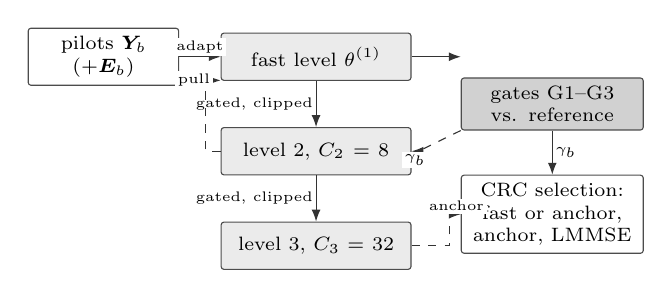
\begin{tikzpicture}[x=1mm,y=1mm]
\node[blk,text width=17mm] (pil) at (0,14) {pilots $\bm Y_b$\\($+\bm E_b$)};
\node[mem,text width=22mm] (l1) at (27,14) {fast level $\theta^{(1)}$};
\node[mem,text width=22mm] (l2) at (27,2) {level 2, $C_2=8$};
\node[mem,text width=22mm] (l3) at (27,-10) {level 3, $C_3=32$};
\node[gat,text width=21mm] (gate) at (57,8) {gates G1--G3\\vs. reference};
\node[blk,text width=21mm] (out) at (57,-6) {CRC selection:\\fast or anchor,\\anchor, LMMSE};
\draw[arr] (pil)--(l1) node[midway,lbl,above]{adapt};
\draw[arr] (l1.east)--(gate.west|-l1.east);
\draw[arr] (gate)--(out) node[midway,lbl,right]{$\gamma_b$};
\draw[arr] (l1)--(l2) node[midway,lbl,left]{gated, clipped};
\draw[arr] (l2)--(l3) node[midway,lbl,left]{gated, clipped};
\draw[darr] (l3.east)--(44,-10)--(44,-6)--(out.west) node[pos=0.6,lbl,above]{anchor};
\draw[darr] (gate.south west)--(40,2)--(l2.east) node[pos=0.5,lbl,below]{$\gamma_b$};
\draw[darr] (l2.west)--(13,2)--(13,11)--(l1.west|-13,11) node[pos=0.5,lbl,left]{pull};
\end{tikzpicture}
\caption{Citadel-Rx. The fast level fits every block; the gates compare its decisions with the
better of LMMSE on the block's pilots and the anchor detector; levels 2 and 3 receive gated, clipped averages of the
faster states; a rejected block is reverted and detected with the anchor; every CRC sub-block
keeps the first passing detection. The anchor is the mean of levels 2 and 3; its two arrows are drawn from one level each.}
\label{fig:arch}
\end{figure}

\subsection{Levels and the Fast Learner}
The adaptable parameters $\theta\in\mathbb{R}^d$ (all DeepSIC weights, $d=67\,632$ for $4\times4$ QPSK)
are kept at $K=3$ levels with periods $C=(1,8,32)$ blocks. The fast level is adapted on every
block by $T=300$ steps of
\begin{align}
\theta&\leftarrow\theta-\eta_b\delta\,\theta\,\bm\phi\bm\phi^{\!\top}\quad\text{(delta-rule decay, per weight matrix)},\label{eq:delta}\\
\theta&\leftarrow\theta-\eta_b\lambda(\theta-a_b)\quad\text{(proximal pull to the anchor)},\label{eq:prox}\\
\theta&\leftarrow\mathrm{Adam}\big(\theta,\nabla_\theta\ell_b(\theta)\big),\label{eq:adam}
\end{align}
with $\ell_b$ the pilot cross-entropy of the stage being adapted, its gradient evaluated before \eqref{eq:delta} and \eqref{eq:prox} are applied (stages are adapted sequentially
\cite{shlezinger2021}), $\bm\phi$ the normalised mean input of the weight matrix (the stage input for
the first layer, the hidden activation for the second; biases are not decayed), and
$a_b=\tfrac12\theta^{(2)}_{b-1}+\tfrac12\theta^{(3)}_{b-1}$ the anchor (weights $w_k=\tfrac12$ in Algorithm~\ref{alg:block}). The step size follows the ratio of the receiver's surprise $S_b=\norm{\nabla_\theta\ell^{\rm det}_b(\theta_{b-1})}^2$ to its moving average $\bar S_b$, where $\ell^{\rm det}_b$ is the pilot cross-entropy of the posteriors of the full detector: $\eta_b=\eta_{\max}\,2r_b/(1+r_b)$ with $r_b=\mathrm{clip}(S_b/\bar S_b,\tfrac18,8)$, so the rate is
bounded by $2\eta_{\max}$.

\subsection{Gated, Clipped Consolidation}
At the end of every period of level $k{+}1$ the level receives the gated mean of the level-$k$
states buffered since its last update, each weighted by the verdict $\gamma_j\in[0,1]$ of its
block (or the mean verdict of its period):
\begin{equation}\label{eq:consol}
\begin{aligned}
\theta^{(k+1)}&\leftarrow\theta^{(k+1)}+\Pi_{\kappa_{k+1}}\!\Big(s\big(m-\theta^{(k+1)}\big)\Big),\\
m&=\frac{\sum_j\gamma_j\theta^{(k)}_j}{\sum_j\gamma_j},\qquad s=\eta^{(k+1)}\min\big(1,\textstyle\sum_j\gamma_j\big),\\
\Pi_\kappa(\bm v)&=\bm v\min\{1,\kappa/\norm{\bm v}\},
\end{aligned}
\end{equation}
with $\eta^{(2)}=1$, $\eta^{(3)}=\tfrac12$, and no update when $\sum_j\gamma_j=0$. The clip $\kappa=(8.5,4.5)$ lies
at or just above the largest clean consolidation increments of levels 2 and 3 on the calibration
runs (\val{clip.calmax2} and \val{clip.calmax3}), so it rarely binds on clean runs (in
\val{clip.cln} consolidations of the clean twins at the headline cell) and limits what any attacked
period can move. The first version of the
receiver divided the gated sum by $\max(1,\sum_j\gamma_j)$; when the verdicts of a period sum to less than one, that is, when nearly all its blocks are
rejected, which is the case under attack, this pulls the level towards the origin instead of
leaving it nearly unchanged, and the update is then not the convex combination that the bounds of
Section~\ref{sec:theory} require. Every result of this paper uses \eqref{eq:consol}.

\subsection{Rejection, Fallback and CRC Selection}
If $\gamma_b<\tfrac12$ the block is rejected: the fast update is reverted, the reverted state enters
the buffer with weight $\gamma_b$, and the data of the block are detected with the anchor, which
the pilots of this block have not changed; attacked blocks that were accepted earlier have entered it through the consolidation (Section~\ref{sec:retention}). Each CRC sub-block of each user then keeps the first of three
detections that passes its CRC: the gate's choice (fast level or anchor), the anchor, and LMMSE on
the least-squares channel estimate. All three are already computed for the gates; when none passes, the gate's choice is kept.

Four optional mechanisms answer specific attacks and are evaluated
with them (Sections~\ref{sec:refdeg}--\ref{sec:retention}). \emph{Abstain}: the block is rejected
and not buffered when the reference itself has degraded. The first version tested the reference's
pass fraction and residual against their running levels on accepted blocks ($z_{\rm a}=4$, binomial floor
on the variance), and on clean runs it tripped and then rejected every later block (Section~\ref{sec:refdeg}). The final version tests
$t_b=\log(r^{\rm v}_b/\hat\sigma^2_b)$, where $r^{\rm v}_b$ is the mean squared residual
$\norm{\bm y_n-\hat{\bm H}_b\bm s_n}^2/N$ over the symbol slots whose decisions the CRC verifies for every
user (the residual of the LMMSE decisions if fewer than 5\% are verified) and $\hat\sigma^2_b$ is the
noise power estimated on the pilots, both per antenna. Without attack both follow the noise power (the data residual also carries the channel-estimation error, and the verified slots leave out the largest noise samples, two offsets that the running level tracks), whatever the
channel, because verified decisions are correct; poisoned pilots inflate $\hat\sigma^2_b$ and energy
on the data inflates $r^{\rm v}_b$. The receiver abstains when $|t_b-\bar t_b|>z_{\rm a}\max(s_b,0.1)$,
with the level $\bar t_b$ and the spread $s_b$ tracked on every non-abstained block, and re-bases the
level after 50 consecutive abstentions, so that a lasting change does not make it abstain indefinitely; in the runs
with a change at block 50 of 100 the re-base can fire only at the last block, so it is not evaluated. An intermediate
version on the residual of the hard LMMSE decisions was dropped after its first test runs: that
residual also follows the decision errors of the reference, which a legitimate redraw to a
worse-conditioned channel raises. \emph{Per-user gating}: G2 is evaluated per user with that user's
pass fractions, and only the users whose test fails revert their networks and fall back to the
anchor (G1 and G3 still judge the block). \emph{Streak recovery}: after five consecutive rejections
a re-fit from the anchor on CRC-verified data, kept if it verifies better than the reference.
\emph{Drift guard}: a pull of level $K$ towards the pre-trained weights by $5\%$ per consolidation.

\begin{algorithm}[t]
\caption{Citadel-Rx, one block $b$}\label{alg:block}
\scriptsize
\begin{algorithmic}[1]
\Require pilots $\bm Y_b$ (possibly poisoned), data $\bm Y^{d}_b$; levels $\theta^{(1..K)}$; buffers; running statistics
\State $a_b\gets\sum_{k\ge2}w_k\theta^{(k)}$; \ $\eta_b\gets\eta_{\max}2r_b/(1+r_b)$
\State reference: $\hat{\bm H}_b$ (LS, AR(1) tracker); $\hat{\bm s}_{\rm mm}$ (LMMSE); $\hat{\bm s}_{a}$ (anchor)
\State $\theta\gets\theta^{(1)}$; $T$ steps of \eqref{eq:delta}--\eqref{eq:adam} on $\bm Y_b$; $\hat{\bm s}_{\rm nn}\gets$ detect$(\theta,\bm Y^d_b)$
\State $\gamma_b\gets\min(\gamma_1,\gamma_2,\gamma_3)$: G1 residual ratio, G2 CRC ratio $F_{\rm nn}/F_{\rm ref}$, G3 innovation
\If{$\gamma_b<\tfrac12$}
\State $\theta\gets\theta^{(1)}$ (revert); \ $\hat{\bm s}\gets\hat{\bm s}_{a}$ (fallback)
\Else
\State $\hat{\bm s}\gets\hat{\bm s}_{\rm nn}$; update the running statistics
\EndIf
\State per user and sub-block: $\hat{\bm s}\gets$ first CRC-passing of $(\hat{\bm s},\hat{\bm s}_a,\hat{\bm s}_{\rm mm})$
\State $\theta^{(1)}\gets\theta$; buffer $(\gamma_b,\theta^{(1)})$; for every $k$ with $(b+1)\bmod C_{k+1}=0$: \eqref{eq:consol}
\State \Return $\hat{\bm s}$
\end{algorithmic}
\end{algorithm}

\subsection{Relative Physics Gates}\label{sec:gates}
The statistics of G1 and G2 are ratios against a reference computed on the same block without labels: the better of the LMMSE detector on the least-squares (LS) pilot estimate $\hat{\bm H}_b$ and the anchor detector. The statistic of G3 is a ratio against its own running level. The ratios are normalised by their moving averages over accepted blocks and passed through a soft step of width $\omega=0.1\tau$ at the threshold $\tau$, which is tightened by up to $30\%$ when $r_b>1$.

\textit{G1, model residual.} With $r(\hat{\bm s})=\tfrac1{N_d}\sum_n\norm{\bm y_n-\hat{\bm
H}_b\hat{\bm s}_n}^2$, the statistic is $r(\hat{\bm s}_{\rm nn})/r(\hat{\bm s}_{\rm ref})$ against
$\tau_1=1.25$.

\textit{G2, CRC pass fraction.} The statistic is the pass fraction $F_{\rm nn}$ of the fast level over that of the reference, $F_{\rm ref}$, against the threshold $\tau_2$ of the design rule of Section~\ref{sec:theory}. The gate is tied to the availability attacker's own objective: an attack that raises the SER lowers the pass fraction. With LDPC code blocks
(Section~\ref{sec:umi}) the CRC after decoding tolerates raw symbol errors, so the pass fraction of
a code block does not follow the design rule. There $F$ is replaced by the virtual pass fraction $(1-\hat p)^L$, and the rule applies unchanged. Here $\hat p$ (the $p$ of the design rule) is the symbol error rate of a detector over all users (per user with per-user gating), measured on the code blocks that decode under a reference, whose re-encoded codewords are taken as the transmitted symbols. When no code block decodes under any reference, the code-block pass fractions are used.

\textit{G3, channel prior.} The statistic is the innovation energy of the LS estimate with respect to its first-order autoregressive, AR(1), prediction (the previous block's estimate, scaled by the channel's correlation on Jakes fading), divided by its running level on accepted blocks, which is floored by its expected value. It is tested against $\tau_3=\max\{4,\chi^2_{0.999}(NU)/(NU)\}$, which is 4 for every array here.

Table~\ref{tab:hyper} gives the provenance of the main settings.

\begin{table}[t]
\centering\caption{Settings and their provenance. Calibration: seeds 0--2 by the rules of
Section~\ref{sec:setup}; first version: set during the development of the first version on seeds
0--4. No setting was chosen on the test seeds 10--19, with two exceptions: the statistic of the final
abstain state, adopted after first test runs of its second version (stated in the table), and the
SED profile of the larger arrays, stretched after test runs with the unstretched one
(Section~\ref{sec:scen}).}\label{tab:hyper}
\scriptsize
\begin{tabular}{@{}L{36mm}L{49mm}@{}}
\toprule
Setting & Value; provenance\\
\midrule
$Q$, MLP width, $T$, $\eta_{\max}$, Adam & 3, $64\cdot$order for QPSK ($=256$), 300, $5\cdot10^{-3}$; reference code released with \cite{raviv2024}, architecture of \cite{shlezinger2021}; width kept at 256 for 16-QAM (not $64\cdot16$, Section~\ref{sec:scen})\\
$K$, $C$ & 3, $(1,8,32)$; first version; ablation in Section~\ref{sec:ablate}\\
$\eta^{(2)},\eta^{(3)}$, $\lambda$, $\delta$ & $1,\tfrac12$, $0.5$, $0.1$; first version; sensitivity of $\eta^{(3)}$, $\lambda$, $\delta$ in Section~\ref{sec:sens}\\
$\tau_1,\tau_3,\omega$, tightening & $1.25$, $4$, $0.1\tau$, $30\%$; first version; sensitivity\\
Surprise clip, rejection threshold, anchor weights, G3 quantile & $[\tfrac18,8]$, $\tfrac12$, $(\tfrac12,\tfrac12)$, $0.999$; first version\\
CRC slack & relative $\rho=1$ with floor $2\cdot10^{-3}$ (first version), or derived $z=5$ (set before calibration); mode chosen by calibration (\val{cal.chosen})\\
$\kappa$ & $(8.5,4.5)$; set before calibration from the clean consolidation increments of earlier records of the calibration configurations; common to all candidates\\
Consolidation rule, CRC selection & \eqref{eq:consol}; correctness fix; CRC selection common to all calibration candidates (ablation in Section~\ref{sec:ablate})\\
Baseline epochs, learning rate, weight decay & tuned on calibration seeds (Section~\ref{sec:setup})\\
Baseline method settings & L2-SP, EWC $10^{-2}$; EMA 0.9; CoTTA restore 0.05; EATA $0.4\ln4$; decision-directed weight 1; drift threshold 2; four median-of-means groups; not tuned (L2-SP also swept, Section~\ref{sec:baselines})\\
Streak $k$, drift guard, abstain fallback, spread floor & 5, $5\%$, $5\%$ verified, $0.1$; one value each, not tuned\\
Abstain (final version) & statistic and re-base after 50 abstentions: adopted after the second version's first test runs (seeds 10--12, A4); $z_{\rm a}=\val{h3.z}$ by calibration; also tested on seeds 15--19, untouched by any choice\\
Second backbone & 512 hidden units; epochs and learning rate tuned on calibration seeds (\val{d8.tuned})\\
Attacker & PGD 20 steps of $0.25\epsilon$, 2 unrolled steps; our implementation of the pilot poisoning of \cite{wu2024}; stronger variants in Section~\ref{sec:adaptive}\\
\bottomrule
\end{tabular}
\end{table}

\section{Retention Bounds}\label{sec:theory}
The bounds are stated for the algorithm as implemented, for a pair of runs on the same channel,
noise and seed, with and without an attack that starts at block $b_0$ (the runs are identical
before $b_0$). Let $n(W)$ be the number of level-$K$ consolidations in $[b_0,b_0+W)$, so
$n(W)\le\lceil W/C_K\rceil$; quantities of the clean run are primed.

\begin{lemma}[convex consolidation]\label{lem:convex}
Without the clip, \eqref{eq:consol} writes the new level-$(k{+}1)$ state as the convex combination
$(1-s)\theta^{(k+1)}+s\,m$ of its old state and the buffered states (for $\sum_j\gamma_j>0$), with $s\le\eta^{(k+1)}\le1$ and $m$ in
their convex hull. With the clip the step is $\tilde s=s\min\{1,\kappa_{k+1}/\norm{s(m-\theta^{(k+1)})}\}\le
s$, and the statement holds with $\tilde s$.
\end{lemma}

\begin{theorem}[retention]\label{thm:retention}
(i) \emph{Design bound.} With the clip, for any perturbations and any gate verdicts,
\begin{equation}\label{eq:design}
D_K(b_0+W-1)\le 2\kappa_K\,n(W).
\end{equation}
(ii) \emph{Structural bound.} Let the two runs buffer the same blocks (always the case without the abstain state) and let $\sum_j\gamma_j>0$ in both at every level-$K$ consolidation of the window. Let $\Delta(W)$ be the largest paired displacement of the buffered
level-$(K{-}1)$ states in the window and, at the $i$-th consolidation, $\bar w_i,\bar w_i'$ the
normalised weights, $\tilde s_i,\tilde s_i'$ the steps taken, $m_i'$ the clean gated mean and $r_i'$
the radius of the clean buffer around it, and $\theta'^{(K)}_i$ the clean level-$K$ state before that consolidation. Then
\begin{multline}\label{eq:struct}
D_K(b_0+W-1)\le\big(\Delta(W)+\Omega(W)\big)\big(1-(1-\eta^{(K)})^{n(W)}\big)\\
+\sum_{i\le n(W)}|\tilde s_i-\tilde s_i'|\,\norm{\theta'^{(K)}_i-m'_i},
\end{multline}
with $\Omega(W)=\max_i\norm{\bar w_i-\bar w'_i}_1r'_i$. With equal verdicts $\Omega=0$; if moreover
the clip binds in neither run, or with the same factor in both, at every consolidation of every level,
then $\tilde s_i=\tilde s_i'$, the sum vanishes, and $\Delta(W)$ is at most the largest paired
fast-level displacement.
\end{theorem}
\begin{proof}
(i) Level $K$ changes only at consolidations, and in each run by at most $\kappa_K$; the drift guard,
when used, multiplies the paired difference by $0.95$. (ii) By Lemma~\ref{lem:convex}, at consolidation $i$,
$\theta^{(K)}_{\rm new}-\theta'^{(K)}_{\rm new}=(1-\tilde s_i)(\theta^{(K)}-\theta'^{(K)})+\tilde s_i(m_i-m'_i)+(\tilde s_i-\tilde s'_i)(m'_i-\theta'^{(K)})$.
Since $\sum_j\bar w_{ij}=\sum_j\bar w'_{ij}=1$, $m_i-m'_i=\sum_j\bar w_{ij}(\theta_j-\theta'_j)+\sum_j(\bar w_{ij}-\bar w'_{ij})(\theta'_j-m'_i)$,
whose norm is at most $\Delta+\Omega$. Iterating $D\leftarrow(1-\tilde s_i)D+\tilde s_i(\Delta+\Omega)+e_i$ from
$D=0$ gives $D\le(\Delta+\Omega)(1-\prod_i(1-\tilde s_i))+\sum_ie_i$, and $\tilde s_i\le\eta^{(K)}$; as in (i), the drift guard only shrinks the paired difference.
\end{proof}
Bound \eqref{eq:design} needs no measured quantity and holds for every attacker of this paper,
including those that pass the gates; its price is that a legitimate change of the channel moves the
slowest level by at most $\kappa_K$ per period. The same argument gives $D_2\le2\kappa_2\lceil W/C_2\rceil$ for $K=3$, so the anchor, which the fallback and the proximal pull use, is displaced by at most $\kappa_2\lceil W/C_2\rceil+\kappa_K n(W)$ after the last block of the window. Bound \eqref{eq:struct} is evaluated on the paired
trajectories in Section~\ref{sec:retention}; it is tighter when the verdicts agree, and it is the
form in which the gate enters: rejected blocks are reverted and enter with weight $\gamma_b$.

\begin{remark}[contraction]\label{rem:contraction}
If the block map satisfied $\norm{\Phi(\theta;\bm Y+\bm E,a)-\Phi(\theta;\bm Y,a)}\le G_\Phi\norm{\bm E}$ and were
jointly $L_\Phi$-Lipschitz in $(\theta,a)$ with $L_\Phi<1$, and if every block of the window were
accepted in both runs with equal verdicts and equal clip factors, so that by Lemma~\ref{lem:convex} the paired displacement of the anchor is at most the largest paired fast displacement so far, the largest fast displacement $\Delta_f$ after $n_W$ attacked blocks of budget $\epsilon$ would satisfy
$\Delta_f\le G_\Phi\epsilon(1-L_\Phi^{n_W})/(1-L_\Phi)$; on a block accepted in one run only, the
displacement can grow by the norm of that run's update, which does not scale with $\epsilon$. The
sufficient condition is $L_\theta+L_a<1$, with $L_\theta$ and $L_a$ the Lipschitz constants of $\Phi$ in $\theta$ and in $a$, whose sum bounds $L_\Phi$ (taken for $\max\{\norm{\theta-\theta'},\norm{a-a'}\}$) from above. Finite-difference probes of the fast learner, which the correction of \eqref{eq:consol} does not change,
give $L_\theta+L_a$ between \val{lip.summin} and \val{lip.summax} for proximal weights $\lambda$ from
\val{lip.lammin} to \val{lip.lammax}, and a stronger search, a finite-difference hill climb on the
input direction for $G_\Phi$ and the largest of 20 random parameter and anchor directions on each
of 10 blocks for $L_\theta$ and $L_a$, gives \val{lip2.summin} to \val{lip2.summax} on the cosine,
Jakes and COST2100 channels at the frozen settings (with $G_\Phi$ of at least \val{lip2.cosine.g}, \val{lip2.jakes.g} and \val{lip2.cost.g} on the three); probes can
only underestimate a Lipschitz constant, so the sufficient condition is not met, and on the cosine channel the probe of $L_\theta$ alone (\val{lip2.cosine.lt}) exceeds one, which excludes $L_\Phi<1$; the contraction argument cannot be used for the
default receiver. The regret bound of the first version, which relied on
it, is withdrawn; a last-layer-adaptable variant, for which the loss is convex, is evaluated in
Section~\ref{sec:scen} without a regret claim.
\end{remark}

\textit{Design rule for the CRC gate.} With i.i.d. symbol errors of probability $p$ in a sub-block of
$L$ symbols and an $r$-bit CRC whose syndrome is uniform on error, $P(\mathrm{pass}\mid
p)=(1-p)^L+2^{-r}(1-(1-p)^L)$. Neglecting the $2^{-r}$ term,
inverting at $F_{\rm ref}$ gives $p_{\rm ref}=1-F_{\rm ref}^{1/L}$, and the rule ``reject if
$F_{\rm nn}/F_{\rm ref}<\tau_2$'' with $\tau_2=\big((1-p_{\rm ref}-\xi)/(1-p_{\rm ref})\big)^{L}$
tolerates an excess error probability $\xi$ over the reference. The gate applies the rule to the ratio normalised by its moving average over accepted blocks (Section~\ref{sec:gates}), so that, to first order, $\xi$ is counted from the fast level's usual error probability, which is that of the reference only when the moving average is one. The relative slack sets
$\xi=\max\{2\cdot10^{-3},\rho\,p_{\rm ref}\}$; the derived slack removes the floor and takes
$\tau_2=\min\{1-z\sigma,\tau_2(\rho p_{\rm ref})\}$, with $\sigma$ the standard deviation of the
normalised pass ratio on accepted blocks, floored by the binomial relative standard deviation $\sqrt{F_{\rm ref}(1-F_{\rm ref})/n_{\rm c}}/F_{\rm ref}$ of the reference pass fraction over the $n_{\rm c}$ CRC checks of the statistic ($n_{\rm c}=nU$ for the block gate, $n_{\rm c}=n$ per user), so the
threshold follows the block length. For $n$ independent sub-blocks, a pass fraction $\hat F$ with expectation $F$ satisfies $P(|\hat F-F|\ge t)\le2e^{-2nt^2}$
\cite{hoeffding1963}. The formula is standard; its use here is to replace a tuned threshold by a
target excess error. In the evaluated receiver that target keeps the first-version values ($\rho=1$, floor $2\cdot10^{-3}$), which were not derived. Here $p$ is the symbol-error probability of a user, pooled over the users by the gate; the SER of Section~\ref{sec:model} counts a slot in which any user is wrong and is therefore at most $U$ times this $p$. The independence of the symbol errors within a sub-block is an assumption that was not checked against the records.

\textit{Model mismatch and G1.} Writing $\bm y_n=\hat{\bm H}\bm s_n+\bm\nu_n+\bm m_n$ with $\bm m_n$ the
mismatch, the residual of a decision with error $\bm e_n$ is $\mathrm{mean}\norm{\hat{\bm H}\bm
e_n}^2+\mathrm{mean}\norm{\bm\nu_n+\bm m_n}^2$ plus a cross term that vanishes if decision errors are
uncorrelated with noise and mismatch. This is an assumption, not a fact: errors occur when the
noise is large. On clean blocks of the $\tanh$ channel at 10\,dB (first-version runs, seeds 0--2)
the normalised G1 statistic has mean \val{g1nl.mean}, 99th percentile \val{g1nl.p99} and maximum
\val{g1nl.max} over \val{g1nl.n} blocks; its largest value at any SNR from \val{g1nl.snrmin} to
\val{g1nl.snrmax}\,dB is \val{g1nl.allmax}, below $\tau_1=1.25$ but above the fully tightened
threshold $1+0.7(\tau_1-1)$, so G1 can reject a clean block of this channel when the surprise is high.

\section{Experimental Protocol}\label{sec:setup}

\textit{Benchmark channel.} The SED channel of the DeepSIC literature (Table~\ref{tab:setup}) is real-valued with deterministic fades, identical for every seed: the seeds change the noise, the symbols and the attack window, and pre-training uses its block-0 matrix at several SNRs. The test seeds therefore do not test a new channel.

\textit{Receivers.} The receivers compared are LMMSE on the least-squares pilot estimate and a Huber-robust version
\cite{huber1964}; online DeepSIC \cite{shlezinger2021}; Meta-DeepSIC \cite{raviv2023};
\emph{CRC-Rollback}, online DeepSIC with the CRC gate G2 at a fixed absolute slack of $0.01$ ($\tau_2=0.99^{L}$, tightened under surprise as in
Section~\ref{sec:gates}), judged against LMMSE only, without CRC selection, and with rollback to the
last accepted weights, and the same with all three gates (the $K=1$ ablation, Section~\ref{sec:ablate},
has Citadel-Rx's gates and selection); online DeepSIC with the CRC selection of Citadel-Rx, which separates
the selection gain from the memory; L2-SP \cite{l2sp2018}, elastic weight consolidation (EWC) with the Fisher information of the pre-training data \cite{ewc2017} and an exponential-moving-average (EMA) teacher \cite{meanteacher2017}; CRC-verified
decision-directed training, which adds the CRC-passing data symbols to the pilots \cite{viterbinet2020,schibisch2018};
an EATA-style receiver (entropy filter and Fisher anchor) \cite{eata2022} and a CoTTA-style receiver (teacher and stochastic restore) \cite{cotta2022}; a drift-detection receiver after \cite{uzlaner2024}, with a simpler statistic, that adapts a user's
modules only when that user's pilot loss, standardised by its running mean and spread, exceeds 2; a
median-of-means gradient receiver (coordinate-wise median of the gradients of four disjoint pilot
groups), which moves the median of \cite{medbn} from the batch-normalisation statistics, which DeepSIC does not have, to the gradient; and a single-memory receiver with the fast learner of
Citadel-Rx and no slow levels \cite{behrouz2025titans}. All DeepSIC receivers share the
architecture and the pre-training. A second backbone replaces DeepSIC in Citadel-Rx, online
training and CRC-Rollback: a fully connected network with one hidden layer of 512 units that
classifies the joint symbol of all users ($4^U=256$ classes) from the received vector, without
interference cancellation \cite{oshea2017,samuel2019}; detection uses its per-user marginals.

\begin{table}[t]
\centering\caption{Simulation setup.}\label{tab:setup}
\scriptsize
\begin{tabular}{@{}L{14mm}L{71mm}@{}}
\toprule
System & $U\times N=4\times4$, QPSK, SNR $10$\,dB; $4\times16$ and $8\times32$ with the SED profile stretched over the array; 16-QAM at 20\,dB (MLP width kept at 256)\\
Block & $N_p=100$ pilot and $N_d=24\,992$ data symbols per user; $N_d=992$ and $4\,992$ (nominally 1000 and 5000), $N_p\in\{32,100\}$ in Section~\ref{sec:scen}\\
CRC & CRC-8 of \cite{ts36212}, $D^8+D^7+D^4+D^3+D+1$; $L=32$; $n=781$ sub-blocks per user and block\\
Channel & SED with per-user cosine fading, gain $0.8+0.2\cos(2\pi b/T_j)$ with $T_j=51,39,33,21$ blocks (users 5--8: 47, 29, 43, 23) \cite{shlezinger2021}; COST2100 traces \cite{liu2012cost} from the code released with \cite{raviv2024}, in calibration\\
Run & 100 blocks (400 and 1000 for A3$^\ast$, 2000 clean); unless stated, a 40-block attack window starting at a block drawn uniformly from 10--50 per seed; fixed windows: 30--69 for calibration and retention, 40--89 for denial, 30--329 and 30--929 for A3$^\ast$\\
Seeds & calibration 0--2; test 10--19 (headline cell, final abstain state), up to 10--14 elsewhere (every table states its seeds), 10 (sensitivity)\\
Coded scene & TR 38.901 UMi at 3.5\,GHz, 1$\times$4 array at 10\,m, users at 20--150\,m with ideal slow power control, 3\,km/h; one block per 1\,ms slot (15\,kHz, 150 PRBs); NR LDPC code blocks (base graph 2, $k=520$, $n=1000$), each with a CRC-24A \cite{ts38212}, scrambled \cite{ts38211}\\
Attacker & A1, after \cite{wu2024}: PGD \cite{madry2018}, 20 steps of $0.25\epsilon$, through 2 unrolled steps, unless stated\\
\bottomrule
\end{tabular}
\end{table}

\textit{Calibration and tuning, fixed in advance.} Online DeepSIC and Meta-DeepSIC are tuned over
300, 100 and 30 adaptation epochs, learning rates $10^{-3}$ and $5\cdot10^{-3}$ and weight decay 0
and $10^{-4}$ on clean runs of the calibration seeds; the setting with the lowest mean clean SER is selected (online DeepSIC:
\val{tune.onlinedeepsic.epochs} epochs, learning rate \val{tune.onlinedeepsic.lr}, weight decay
\val{tune.onlinedeepsic.wd}; Meta-DeepSIC: \val{tune.metadeepsic.epochs}, \val{tune.metadeepsic.lr},
\val{tune.metadeepsic.wd}), and every receiver built on online DeepSIC uses its setting (the drift-detection and median-of-means
receivers, first run at the reference 300 epochs and learning rate $5\cdot10^{-3}$, were re-run with it
for the tables); the baselines' own method settings are not tuned (Table~\ref{tab:hyper}). Citadel-Rx
has three candidates: the relative CRC slack, the derived CRC slack, and the relative slack with a fast level that is restarted from the anchor every block and whose update per block is projected onto a ball of radius 13. All three use the CRC selection, the clip $\kappa$ and \eqref{eq:consol}. The rule, fixed before the runs, selects the candidate with the lowest mean of the clean SER, the A1 window SER at SIR 0\,dB and the A1 window SER on COST2100, among candidates with at most $2\%$ clean false rejections (Table~\ref{tab:cal}). The chosen settings are written to a file
by the rule and read by every test run. The second campaign added two choices, again on seeds 0--2
by rules fixed before any test run of the features: the abstain threshold $z_{\rm a}$ is the smallest of
3, 4, 5, 6 and 8 with at most $2\%$ abstentions on the clean blocks of calibration runs that never
abstain (\val{h3.calblocks} blocks; chosen $z_{\rm a}=\val{h3.z}$, largest deviation
\val{h3.calmax}), and online training on the second backbone is tuned over 30 and 100 epochs and
learning rates $10^{-3}$ and $5\cdot10^{-3}$ like online DeepSIC (\val{d8.tuned}); Citadel-Rx keeps
all its frozen settings on the second backbone and in the coded scene.

\textit{Statistics.} Within a run, consecutive blocks are correlated (a decorrelation length of
\val{p1.citadel.wb0.decor} blocks for the excess SER at the headline cell), so intervals are 95\%
moving-block bootstrap intervals \cite{kunsch1989} (percentile intervals from 4000 resamples) that resample seeds and then, within each seed, stretches
of consecutive blocks of twice the decorrelation length (at least five blocks), wrapped around the end of the series. Tests are at the seed level: an exact two-sided Wilcoxon
signed-rank test on the per-seed means \cite{wilcoxon1945}, whose smallest attainable $p$ with ten
seeds is $0.002$, Holm-corrected over the four baselines of a column \cite{holm1979}. Rejection and false-rejection rates pool the blocks of all seeds of a cell; their Wilson intervals at the headline cell \cite{wilson1927} treat these blocks as independent and are too narrow if the verdicts of consecutive blocks are correlated.

\textit{Reproducibility.} The first campaign ran on an Apple M4 laptop (ten cores, eight runs at a
time) and a 4-core cloud machine, the second on 4-core cloud machines, every run single-threaded,
with disjoint sets of runs. Runs used PyTorch 2.14.1, NumPy 2.5.3 and SciPy 1.18.1 with one CPU thread per run; each attacked run and its clean twin ran on one machine (or, for re-runs, on a machine that reproduces the twin block for block before the window). Times per block come from the M4 runs and compare receivers only roughly;
machine-independent costs are counted in multiply-accumulates. Every record stores its configuration,
seed, code version and timings.
Pre-training is cached by configuration, seed, code and random-number state, and a cached run reproduces the uncached run exactly (the repository's tests compare the two). Three commands re-run the two campaigns, and
\texttt{make paper} recomputes every number, table and figure of this paper from the records and
rebuilds it (README, section Reproducibility).

\begin{table}[t]
\centering\caption{Calibration of Citadel-Rx on seeds 0--2 (SER). Score: mean of the clean, A1 and
COST2100 A1 columns.}\label{tab:cal}
\scriptsize
\begin{tabular}{@{}L{19mm}cccccl@{}}
\toprule
Candidate & Clean & \thead{A1\\window} & \thead{COST2100\\A1} & \thead{False\\rej.} & Score & \\
\midrule
\tab{calibration}
\bottomrule
\end{tabular}
\end{table}

\section{Results}\label{sec:results}

\subsection{Headline Comparison}\label{sec:headline}
\begin{table*}[t]
\centering\caption{Excess SER (attacked minus matched clean run, attack window) at the headline
cells, test seeds; 95\% moving-block interval at white-box SIR 0\,dB. Seeds 10--19 for WB $0$\,dB, Clean, Rej.\ and False rej., seeds 10--14 for
the other columns. Clean: SER of the clean twins over blocks 5--99. Rejection of the poisoned blocks and false
rejection on the clean twins, by the gates of Citadel-Rx and of CRC-Rollback, at white-box SIR 0\,dB.
Never adapts: the pre-trained DeepSIC without test-time training (\val{p1.frozen_deepsic.wb0.n} seeds);
ML: exhaustive maximum-likelihood detection with the LS channel estimate; both were run at white-box
SIR 0\,dB only.}\label{tab:p1}
\scriptsize
\begin{tabular}{@{}lcccccccc@{}}
\toprule
Receiver & Clean & WB $-10$\,dB & WB $0$\,dB & WB $+10$\,dB & Transfer $0$\,dB & Jamming $0$\,dB & Rej. & False rej.\\
\midrule
\tab{p1}
Never adapts & \val{p1.frozen_deepsic.wb0.clean} & -- & \val{p1.frozen_deepsic.wb0.excess} \val{p1.frozen_deepsic.wb0.ci} & -- & -- & -- & -- & --\\
ML, LS estimate & \val{p1.ml.wb0.clean} & -- & \val{p1.ml.wb0.excess} \val{p1.ml.wb0.ci} & -- & -- & -- & -- & --\\
\bottomrule
\end{tabular}
\end{table*}

\begin{table}[t]
\centering\caption{Paired seed-level comparison, Citadel-Rx minus baseline: attack-window SER at
white-box SIR 0\,dB and clean SER (relative change), exact Wilcoxon $p$, Holm-corrected over the
four baselines.}\label{tab:paired}
\scriptsize
\begin{tabular}{@{}lccccc@{}}
\toprule
Baseline & Seeds & $\Delta$ window SER & $p$ & $\Delta$ clean SER & $p$\\
\midrule
\tab{p1_paired}
\bottomrule
\end{tabular}
\end{table}

\begin{figure}[t]
\centering
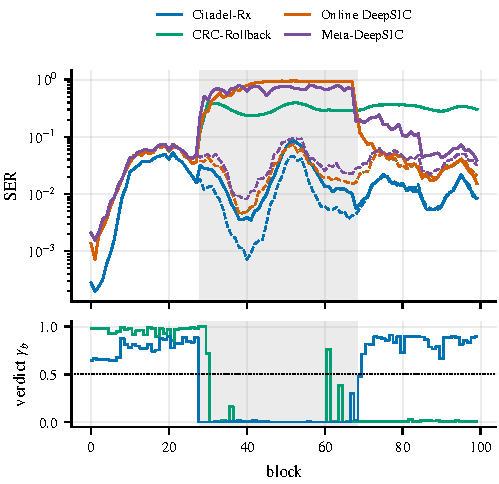
\includegraphics[width=\columnwidth]{fig_rev_trace}
\caption{Test seed 10, white-box A1 at SIR 0\,dB in the shaded window. Top: SER per block of the
attacked runs (solid) and their clean twins (dashed). Bottom: gate verdict $\gamma_b$ of
CRC-Rollback and Citadel-Rx; a block is rejected below $\tfrac12$.}
\label{fig:trace}
\end{figure}

Table~\ref{tab:p1} contains the main result. Under white-box A1 at SIR 0\,dB the attack raises the
SER of Citadel-Rx in the attack window by \val{p1.citadel.wb0.excess} over its clean twin (95\%
interval \val{p1.citadel.wb0.ci}; seed means from \val{p1.citadel.wb0.smin} to
\val{p1.citadel.wb0.smax}), and that of tuned online DeepSIC by \val{p1.online_deepsic.wb0.excess}.
The excess of Citadel-Rx is small but not zero: it is positive on \val{p1.citadel.wb0.spos} of \val{p1.citadel.wb0.n}
seeds (exact Wilcoxon $p=\val{p1.citadel.wb0.p}$). The gates reject \val{p1.citadel.wb0.rejk}
poisoned blocks (95\% Wilson interval \val{p1.citadel.wb0.rejci}) and \val{p1.citadel.wb0.frejk}
clean blocks of the clean twins (\val{p1.citadel.wb0.frejci}). Of the adapting receivers, Citadel-Rx has the
lowest excess, also at SIR $-10$ and $+10$\,dB and under transfer (\val{p1.citadel.wbm10.n} seeds each); the closest
baseline, CRC-Rollback at $+10$\,dB, has \val{p1.crc_rollback.wb10.excess} against \val{p1.citadel.wb10.excess}. Over the blocks after the
window (30, or fewer when the window ends late in the run) the excess of Citadel-Rx is \val{p1.citadel.wb0.post}; online DeepSIC keeps \val{p1.online_deepsic.wb0.post}, CRC-Rollback \val{p1.crc_rollback.wb0.post}, and Meta-DeepSIC, whose meta-training buffer keeps poisoned pilots for 20 blocks after the attack, \val{p1.meta_deepsic.wb0.post}. Fig.~\ref{fig:trace}
shows one seed.

Paired seed by seed (Table~\ref{tab:paired}), Citadel-Rx has the lower window SER against each of
the four baselines on every seed (Holm-corrected $p=\val{cmp.online_deepsic.patt}$, the smallest
attainable with ten seeds and four tests), and also the lower clean SER,
\val{cmp.online_deepsic.clnpct}\% below that of tuned online DeepSIC. Most of the clean gain,
\val{sel.share}\%, comes from the per-sub-block CRC selection rather than from the memory: online
DeepSIC with the same selection has a clean SER of \val{p1.online_select.wb0.clean}, against
\val{p1.online_deepsic.wb0.clean} without it and \val{p1.citadel.wb0.clean} for Citadel-Rx, and
the selection does not protect online DeepSIC (excess \val{p1.online_select.wb0.excess}). The
jamming column is a control, not an attack these receivers are built to resist: at the same SIR,
jamming spreads its power over the data symbols, \val{jam.energyratio} times the energy of the
pilot attack, and raises the SER of every receiver by about the same amount (\val{p1.jam.exmin}
to \val{p1.jam.exmax}); Citadel-Rx rejects \val{p1.citadel.jam.rejk} of the jammed blocks, whose
pilots are clean.

Two reference receivers, run at white-box SIR 0\,dB only, bracket these results
(Table~\ref{tab:p1}). The pre-trained DeepSIC that never adapts is immune to poisoning by
construction (excess \val{p1.frozen_deepsic.wb0.excess}) but has a clean SER of
\val{p1.frozen_deepsic.wb0.clean} on every block, attacked or not, against \val{p1.citadel.wb0.clean}
for Citadel-Rx: test-time learning is what lowers the clean SER, and the gates are what keep the cost of
poisoning small. Exhaustive maximum-likelihood (ML) detection with the LS channel estimate has the
lowest clean SER of all (\val{p1.ml.wb0.clean}), but its channel estimate is taken from the poisoned
pilots, and under the same A1, crafted through the online DeepSIC surrogate rather than tailored to
ML, its excess is \val{p1.ml.wb0.excess}.

\subsection{Failure of Rollback With a Single Memory}\label{sec:c1}
CRC-Rollback is online DeepSIC with the CRC gate G2 at a fixed slack of $0.01$ ($\tau_2=0.99^{L}$),
without CRC selection, and with rollback to the last accepted weights. Under every white-box and
transfer attack of Table~\ref{tab:p1} its excess is several times that of Citadel-Rx, and at SIR 0
and $-10$\,dB and under transfer it does not recover after the window (\val{p1.crc_rollback.wb0.post},
\val{p1.crc_rollback.wbm10.post}, \val{p1.crc_rollback.tr0.post}); at $+10$\,dB it does
(\val{p1.crc_rollback.wb10.post}). The cause is the reference (Fig.~\ref{fig:trace}). The only reference of CRC-Rollback is
LMMSE on the least-squares estimate from the same pilots, and the attack degrades that estimate:
on attacked blocks the reference passes a fraction \val{c1.crc.refatt} of the CRCs, against
\val{c1.crc.refcln} on the same blocks of the clean twin. A poisoned fast level that is merely less
bad than this reference passes the relative test: the first attacked block was accepted on
\val{c1.crc.first0} of \val{c1.crc.nseeds} seeds (\val{c1.crc.acc} attacked blocks accepted in
all). The accepted state then becomes the rollback state; a later update starts from the last accepted state and, in most
blocks, fails the test and is reverted to it. After the attack the receiver rejects a fraction
\val{c1.crc.postrej} of the clean blocks, and over the last ten blocks of the run its excess SER is
still \val{c1.crc.endex}. Rollback with all three gates fails in the same way (\val{c1.rag.nseeds} seeds:
\val{c1.rag.acc} attacked blocks accepted, excess \val{c1.rag.endex} at the end of the run), and so
does Citadel-Rx with its own gates, relative slack and CRC selection but one memory ($K=1$: excess
\val{ab.K1.excess} in the attack window; Section~\ref{sec:ablate}).

Citadel-Rx compares the fast level with the better of LMMSE and the anchor detector, which detects
the data with the slow memory and does not use the pilots of the block. Under attack this
reference passes \val{c1.cit.refatt} of the CRCs (\val{c1.cit.refcln} on the clean twin) while the
poisoned fast level passes \val{c1.cit.nnatt}; \val{c1.cit.acc} attacked blocks were accepted, on
\val{c1.cit.seedsacc} of the \val{c1.cit.nseeds} seeds, and the excess over the last ten blocks
is \val{c1.cit.endex}. The two parts of the principle depend on each other: the gate protects the
memory, and it can only do so because it judges against the memory.

\subsection{Attacks Built Against the Defence}\label{sec:adaptive}
\begin{table}[t]
\centering\caption{Attacks built against the defence, SIR 0\,dB unless stated, test seeds 10--14 (seeds per row).
$^{a}$Soft gates, unroll 10, PGD 50, 2 restarts, EOT over 2 noise draws; $^{b}$the same without soft
gates, which online DeepSIC does not have. With as many antennas as the receiver, the rank-4 physical
attacker reaches every perturbation: it is A1, and its runs are identical to those of the A1 row of
Table~\ref{tab:peruser}. Exact gates: the soft-gate perturbation at \val{orc.ncand} scales, each tried
on an exact copy of the receiver; highest SER sends the most damaging candidate, accepted only the most
damaging candidate the gates accept (seeds 10, 11, 13 and 14). CSI: channel state information.}\label{tab:attacks}
\scriptsize\setlength{\tabcolsep}{2.5pt}
\begin{tabular}{@{}L{20mm}L{12mm}cccc@{}}
\toprule
Attack & Receiver & Seeds & \thead{Excess SER\\{}[95\% CI]} & \thead{Window\\SER} & Rej.\\
\midrule
\tab{attacks}
\bottomrule
\end{tabular}
\end{table}
Every attack of Table~\ref{tab:attacks} was built against the defence, white-box unless stated
(the grey-box attacker knows the defence and its settings, not its weights; the query attacker only
its NACK feedback), and run on test seeds 10--14. Against Citadel-Rx at SIR 0\,dB the \val{atk.cit0.n} attacks, among them the rank-4 physical attacker, which is plain A1 (see the caption), give excess SERs between \val{atk.cit0.exmin} and \val{atk.cit0.exmax}, with rejection rates between \val{atk.cit0.rejmin} (the accepted-only exact-gate run, below) and 1. Plain A1 on the same seeds gives \val{h7.citadela1.excess} to \val{ab.complete.excess} (two sets of runs, on different machines). Deeper unrolling, more steps and restarts, the soft-gate objective with the thresholds and running statistics of G1 and G2 (G3 and the tightening are not modelled), expectation over noise, a Citadel-Rx surrogate, a search on the NACK feedback (one query per attacked block, so not a converged search; Table~\ref{tab:knowledge}) and a budget on the users' signal energy alone get about as few poisoned blocks accepted as plain A1 (rejection at least \val{atk.citadelsigbudgetsir0.rej}, against \val{ab.complete.rej} and \val{h7.citadela1.rej} for A1). So does a physical attacker with two or four antennas, also when its channel estimate is in error (at least \val{atk.b1citadelM2csi001sir0.rej}). A physical attacker with a single antenna gets more poisoned blocks accepted (\val{atk.citadelM1sir0.rejk} rejected) and gives the lowest excess of the full-budget attacks at SIR 0\,dB (\val{atk.citadelM1sir0.excess}). At SIR 10\,dB the excess is
\val{atk.cit10.exmin} to \val{atk.cit10.exmax}. The \val{atk.onl0.n} of these attacks that were also run against online DeepSIC (Combined$^{b}$ in place of
Combined$^{a}$) raise its SER by
\val{atk.onl0.exmin} (rank-1 physical attacker) to \val{atk.onl0.exmax}. All but the accepted-only exact-gate run used their full budget, and with four or five seeds
their excess is not distinguishable from plain A1; what the table shows is that none of these attacks brings Citadel-Rx near the excess of the undefended receivers.

When the gates reject nearly every attacked block, the excess depends on the power of the pilot
perturbation (SIR 0 against 10\,dB), not on how it was optimised: it is the price of rejecting a
block with poisoned pilots; an attack that also reaches the data and gets more blocks accepted costs more
(Section~\ref{sec:refdeg}). The data of the window are detected with the anchor, which has not adapted to the
block, and the LMMSE alternative of the CRC selection uses the poisoned channel estimate (its pass
fraction falls from \val{gate.lmmsecln} on the clean twin to \val{gate.lmmseatt} on attacked
blocks). On the poisoned blocks at the headline cell, the verdict of G2 on its own is below one half
for \val{gate.g2}\% of them, that of G1 for \val{gate.g1}\% and that of G3 for \val{gate.g3}\%: the
decision-level gates G1 and G2 account for the rejections, and G3 flags few poisoned blocks at its threshold.

The exact-gate attacker removes the surrogate's approximations of the gates. It scales the soft-gate
perturbation by each of \val{orc.ncand} factors and tries every candidate on an exact copy of the
receiver, which predicted the receiver's verdict and SER exactly on \val{orc.acc.exact} attacked
blocks (seeds 10, 11, 13 and 14). Sending the most damaging candidate, it always sent the full
perturbation, which the gates rejected (\val{orc.maxser.sentacc} accepted), so that run equals the
soft-gate run block for block on the same seeds. Sending the most damaging candidate that the gates
accept, it found one in \val{orc.acc.anyacc} attacked blocks, at a mean scale of \val{orc.acc.scale}
of the budget; the excess was \val{atk.citadeloracleaccsir0.excess} in the window and
\val{atk.citadeloracleaccsir0.post} after it. The gates can therefore be passed, but in this search only by
perturbations small enough to leave almost no excess after the attack. The search covers only the
scale of one optimised direction, not every perturbation the gates would accept.

\subsection{Attacks on the References and on Adaptation}\label{sec:refdeg}
\begin{table}[t]
\centering\caption{Joint pilot and data attack on the references (A4), white-box SIR 0\,dB, 6 PGD
steps over all data sub-blocks, test seeds 10--14 (rows marked 15--19: seeds 15--19; rows marked 1st: seeds 10 and 11), with and
without the abstain state
(first version: rejects every block of its clean runs as well, see text); one row with 20 PGD steps;
jamming controls with the data power of A4.}\label{tab:refdeg}
\scriptsize
\begin{tabular}{@{}L{12mm}L{12mm}cccc@{}}
\toprule
Attack & State & Seeds & \thead{Excess SER\\{}[95\% CI]} & \thead{Window\\SER} & Rej.\\
\midrule
\tab{refdeg}
\bottomrule
\end{tabular}
\end{table}
\begin{table}[t]
\centering\caption{Abrupt channel redraw at block 50, without and with the denial-of-adaptation
spoof on blocks 40--89 (SIR 10\,dB), and a 6\,dB SNR drop at block 50; test seeds 10--14. SER after
the change (no attack), false rejection after it, excess SER of the spoof in and after its window,
SER after the SNR drop.}\label{tab:deny}
\scriptsize
\begin{tabular}{@{}L{17mm}cccccc@{}}
\toprule
Receiver & Seeds & \thead{SER after\\redraw} & \thead{False\\rej.} & \thead{Spoof\\excess} & \thead{After\\spoof} & \thead{SER after\\drop}\\
\midrule
\tab{deny}
\bottomrule
\end{tabular}
\end{table}
\begin{table}[t]
\centering\caption{Denial of adaptation as intended: white-box A1 at SIR 0\,dB on blocks 40--89 while
the channel is redrawn at block 50, test seeds 10--14. Rejection of the attacked blocks, SER after the
redraw without attack, excess SER in and after the attack, and streak-recovery re-fits tried/kept. The runs without attack are not those of
Table~\ref{tab:deny}: each ran on the machine of its attacked run, and on seeds 10 and 11 that machine
differs between the two tables (SER after the redraw for Citadel-Rx \val{b3.citadel.after} here,
\val{deny.citadel.after} there).}\label{tab:deny2}
\scriptsize
\begin{tabular}{@{}L{17mm}cccccc@{}}
\toprule
Receiver & Seeds & Rej. & \thead{SER after\\redraw} & \thead{Excess in\\window} & \thead{Excess\\after} & \thead{Re-fits\\tried/kept}\\
\midrule
\tab{deny2}
\bottomrule
\end{tabular}
\end{table}
\begin{table}[t]
\centering\caption{Per-user gating against an attack on one user's pilots (A2, user 1) and against
A1, white-box SIR 0\,dB, test seeds 10--14: excess SER of all users and of user 1; rejection of the
attacked blocks (block gate) or reverts of user 1 / of the other users (per-user gate).}\label{tab:peruser}
\scriptsize\setlength{\tabcolsep}{2.5pt}
\begin{tabular}{@{}L{8mm}L{12mm}cccc@{}}
\toprule
Attack & Receiver & Seeds & \thead{Excess SER\\{}[95\% CI]} & \thead{Excess SER\\user 1} & \thead{Rej. or\\reverts}\\
\midrule
\tab{peruser}
\bottomrule
\end{tabular}
\end{table}
A4 splits the attacker's power between the pilots and the data so that the references the gates
compare against degrade together with the fast level (Table~\ref{tab:refdeg}). At the headline
setting and without a channel redraw, it gives Citadel-Rx the largest excess SER of the attacks on
its pilots and references; jamming the data (a control), attacks during a channel redraw
(Tables~\ref{tab:deny} and~\ref{tab:deny2}) and the settings where Citadel-Rx fails (16-QAM and the
coded scene, Sections~\ref{sec:scen} and~\ref{sec:umi}) give more. With a quarter of the power on the pilots, the
reference passes \val{a4.025.refatt} of the CRCs on attacked blocks (\val{a4.025.refcln} on the
clean twin), close enough to the poisoned fast level (\val{a4.025.nnatt}) that only
\val{a4.025.rejk} attacked blocks are rejected, and the excess SER is \val{a4.025.excess}, against
\val{h7.citadela1.excess} to \val{ab.complete.excess} for A1 on the same seeds; with three quarters on the pilots it is
\val{a4.075.excess}. More optimisation raises the excess, with overlapping intervals: with 20 PGD steps instead of 6 the
excess at $\alpha=0.25$ is \val{b2.a4pgd20.excess} and \val{b2.a4pgd20.rejk} attacked blocks are
rejected, against \val{a4.025.excess} and \val{a4.025.rejk} with 6 steps, so the 6-step rows may understate this attacker. Its surrogate models G1 against LMMSE only and G2, with untightened thresholds, and omits G3. The A4 rows therefore describe this attacker, not every joint attacker; more than 20 PGD steps and, for A4, an attacker with exact gates were not run. An attacker that reaches the data does far more harm by jamming them: the same data power as
noise raises the SER by \val{a4.jam025} and \val{a4.jam075} for $\alpha=0.25$ and $0.75$.

The abstain state is meant to answer A4. Its first version did not work: its running statistics
were updated only on accepted blocks and its variance floor was binomial over thousands of CRC
checks, so the fading of the channel alone, which lowers the reference pass fraction from
\val{abs.ref0} to \val{abs.reflock}, tripped it at block \val{abs.lockmin}--\val{abs.lockmax}, and
from then on it rejected every block, clean or attacked (\val{abs.rejk} blocks of its clean twins;
the lower excess of these rows in Table~\ref{tab:refdeg} is that of a receiver that no longer adapts
in either run). The final version (Section~\ref{sec:citadel}) does not trip on clean runs without a channel redraw: it abstained on \val{h3.cleanabstk} clean blocks of seeds 10--14, on \val{h3x.cleanabstk} of
the fresh seeds 15--19 and on \val{h3.snrdrop.abstk} of the blocks after a 6\,dB SNR drop (after the
drop no slot is verified for every user, so there the statistic is that of the LMMSE decisions). It abstains on
every attacked block of A1 and of A4 at $\alpha=0.75$, whose energy on the pilots inflates the noise
estimate, and on \val{h3.a4025.abst}\% of those of A4 at $\alpha=0.25$ on seeds 10--14
(\val{h3x.a4025.abst}\% on seeds 15--19). It lowers the excess of A4, with overlapping intervals, to near
that of A1 with the same state: \val{h3.a4025.excess} and \val{h3.a4075.excess} on seeds
10--14, against \val{a4.025.excess} and \val{a4.075.excess} without it and \val{h3.a1.excess} for A1 (on seeds 15--19,
\val{h3x.a4025.excess} and \val{h3x.a4075.excess}, against \val{h3x.a1.excess} for A1). After a legitimate redraw it abstains on
\val{h3.redraw.abst} of the 50 remaining blocks on average (\val{h3.redraw.n} seeds) and on all of
them on \val{h3.redraw.nall}: when the
CRCs of one user fail after the redraw, no symbol slot is verified for every user (the verified
fraction falls from \val{h3.redraw.verbefore} to \val{h3.redraw.verafter}), the statistic falls back
to the residual of the LMMSE decisions, and that residual follows their errors. On the seeds where it abstains on every remaining block, the
re-base after 50 consecutive abstentions falls on the last block of the run, so these runs do not
test it. With the final abstain state the SER over the blocks after the redraw is \val{h3.redraw.after}, against \val{deny.citadel.after} without it (Table~\ref{tab:deny}; the two sets of runs are not paired). The final version is
therefore not a usable defence either; a residual on the verified symbols of each user is the next
step.

An abrupt channel redraw at block 50 is a legitimate change that the gates must not suppress
(Table~\ref{tab:deny}). After it Citadel-Rx rejects a fraction \val{deny.citadel.frej} of the clean
blocks and its SER over the remaining blocks is \val{deny.citadel.after}, against
\val{deny.onlinedeepsic.after} for online DeepSIC and \val{deny.lmmse.after} for LMMSE: the gates
slow the re-adaptation, a cost of the defence. After a 6\,dB SNR drop, which the receivers are not
told about, all three are close (\val{deny.citadel.drop}, \val{deny.onlinedeepsic.drop},
\val{deny.lmmse.drop}). The denial spoof did not achieve its aim of tripping the gates on every
block: they rejected fractions between \val{deny.citadel.rejattmin} and \val{deny.citadel.rejattmax}
of the spoofed blocks on the \val{deny.citadel.n} seeds. It acted instead as an accepted perturbation during the change,
raising the SER in its window by \val{deny.citadel.excess} for Citadel-Rx,
\val{deny.onlinedeepsic.excess} for online DeepSIC and \val{deny.lmmse.excess} for LMMSE; in the ten
blocks after it, the excess was \val{deny.citadel.post} for Citadel-Rx and
\val{deny.onlinedeepsic.post} for online DeepSIC. Streak recovery was attempted
\val{deny.streak.attempts} times in these runs and kept \val{deny.streak.accepted} times, changing
\val{deny.streak.ndiff} of \val{deny.streak.nruns} runs.

Denial as intended needs an attack that the gates reject on nearly every block. Strong poisoning does that:
A1 at SIR 0\,dB on blocks 40--89, while the channel is redrawn at block 50 (Table~\ref{tab:deny2}),
is rejected on \val{b3.citadel.rej} of the attacked blocks, so Citadel-Rx does not adapt to the new
channel while the attack lasts. It pays \val{b3.citadel.win} in excess SER in the window and still
\val{b3.citadel.post} in the ten blocks after it, against \val{b3.onlinedeepsic.win} in the window
for online DeepSIC, which adapts to the poisoned pilots, and \val{b3.lmmse.win} for LMMSE. Streak
recovery is meant for this case: it re-fitted from the anchor on CRC-verified data
\val{b3.citadelstreak.att} times and kept \val{b3.citadelstreak.acc} of these re-fits, and the
excess was \val{b3.citadelstreak.win} in the window and \val{b3.citadelstreak.post} after it, with \val{b3.citadelstreak.rej} of the attacked blocks rejected. Table~\ref{tab:deny2} has no intervals, so with \val{b3.citadelstreak.n} seeds the reduction is a point estimate, and most of the cost remains. White-box attacks at SIR 10\,dB are also rejected on nearly every block when the channel is not redrawn (Table~\ref{tab:attacks}), so denial may need less power than this; the weakest perturbation that the gates still reject, which sets the attacker's cost of denial, was not searched for, and denial was not run during an SNR drop.

\textit{An attack on one user.} Per-user gating is meant for an attacker who poisons the pilots of
one user only (A2, Table~\ref{tab:peruser}). It does not help here: the excess SER is \val{h7.citadelperusera2.excess} with it and \val{h7.citadela2.excess} without. A2 perturbs the received pilots, which the networks of all users take as input. The block-level gates G1 and G3 reject the whole block on \val{h7.citadelperusera2.rej} of the attacked blocks, and on most of the others the G2 test of the other users also fails, so the other users are reverted on \val{h7.citadelperusera2.revoth} of the attacked blocks and the attacked user on \val{h7.citadelperusera2.revtgt}. On clean blocks \val{h7.citadelperusera2.revclean} of the user updates are reverted. Under A1, which poisons all users, per-user gating gives \val{h7.citadelperusera1.excess}, against \val{h7.citadela1.excess} without it.

\subsection{Retention Under a Slow Small-Budget Attack}\label{sec:retention}
\begin{table}[t]
\centering\caption{Retention of the slowest level: paired displacement $D_K$ against the structural
bound \eqref{eq:struct} and the design bound \eqref{eq:design}, each the largest value in the window,
averaged over seeds; in every run $D_K$ is below both bounds at every block of the window. A1: paired runs with level snapshots, fixed window 30--69, seeds 10--14. A3$^\ast$:
blocks 30--329 of 400 (900 blocks: 30--929 of 1000), perturbation norm relative to the received
pilots, seeds 10--11; with two seeds an interval reflects mostly the variation between blocks, not between seeds.}\label{tab:retention}
\scriptsize
\begin{tabular}{@{}L{14mm}cccccc@{}}
\toprule
Attack & Seeds & \thead{Excess SER\\{}[95\% CI]} & Rej. & $D_K$ & Struct. & Design\\
\midrule
\tab{retention}
\bottomrule
\end{tabular}
\end{table}
\begin{figure}[t]
\centering
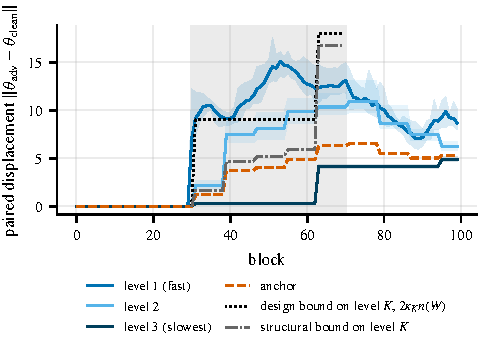
\includegraphics[width=\columnwidth]{fig_rev_p4_paired_a1_sir0_clip}
\caption{Paired displacement of every level and of the anchor under A1 at SIR 0\,dB, window 30--69
shaded (mean over seeds 10--14; for the levels, band from the smallest to the largest seed). The
design bound \eqref{eq:design} and the structural bound \eqref{eq:struct} apply to the slowest level
only; the structural bound is drawn as the largest over the seeds, Table~\ref{tab:retention} gives
its mean.}
\label{fig:retention}
\end{figure}

Table~\ref{tab:retention} and Fig.~\ref{fig:retention} give the paired displacement for the A1 runs
with level snapshots. The largest displacement of the slowest level in the window is
\val{ret.p4sir0.DK} at SIR 0\,dB and \val{ret.p4sir10.DK} at 10\,dB, below the structural bound
(\val{ret.p4sir0.struct} and \val{ret.p4sir10.struct}) and the design bound (\val{ret.p4sir0.design}),
all means over seeds of the largest value in the window; on every seed $D_K$ stays below both bounds
at every block of the window. After the window $D_K$ rises once more, at the next consolidation of the slowest level (Fig.~\ref{fig:retention}), to \val{ret.p4sir0.DKrun} at SIR 0\,dB and \val{ret.p4sir10.DKrun} at 10\,dB (means over seeds of the largest value in the run), below the design bound with the consolidations counted to the end of the run (\val{ret.p4sir0.designrun}); the table and the bounds drawn cover the window only. The anchor, with which rejected blocks are detected, is displaced by up to \val{ret.p4sir0.anchor} in the window (mean over seeds of the largest value). The displacement of the slowest level is not a footprint the attack left in the memory.
Over the window the slowest level of the clean run moved by \val{ret.p4sir0.movcln} and that of the
attacked run by \val{ret.p4sir0.movadv}, in nearly the same direction (cosine
\val{ret.p4sir0.movcos} between the two movements). Rejected blocks enter the consolidation with
weight $\gamma_b\approx0$, so the attacked memory follows the channel more slowly: it moved
\val{ret.p4sir0.movpct}\% as far as the clean memory at SIR 0\,dB and \val{ret.p4sir10.movpct}\%
at 10\,dB, and $D_K$ measures that lag.

\begin{figure}[t]
\centering
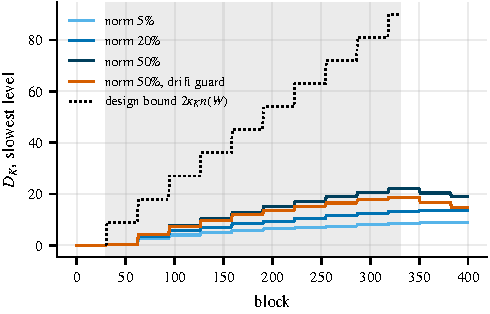
\includegraphics[width=\columnwidth]{fig_rev_drift}
\caption{A3$^\ast$ on blocks 30--329 (shaded): paired displacement of the slowest level for each
perturbation size, and at 50\% also with the drift guard (mean over seeds 10--11, band from the smaller to the larger seed), and the design
bound \eqref{eq:design}; the structural bounds \eqref{eq:struct} are in Table~\ref{tab:retention}.}
\label{fig:drift}
\end{figure}

A3$^\ast$ spreads its perturbation over 300 of 400 blocks, each optimised for the soft-gate objective
so that it is accepted (Table~\ref{tab:retention}, Fig.~\ref{fig:drift}). With a norm of 5\% of that of the
received pilots (SIR \val{ret.p8e005.sir}\,dB) it succeeds: \val{ret.p8e005.rejk} attacked blocks
are rejected. This is the case the retention bounds are for, but not their worst case: A3$^\ast$ optimises each block on its own for an accepted data loss, and its objective has no term for the displacement of the slow level and no target common to its blocks. An attacker that maximises $D_K$ subject to acceptance was not run. Over the window the slowest level of
the attacked run moved as far as that of the clean run (\val{ret.p8e005.movadv} and
\val{ret.p8e005.movcln}), in nearly the same direction (cosine \val{ret.p8e005.movcos}); their paired
displacement reached \val{ret.p8e005.DK}, below the structural bound (\val{ret.p8e005.struct}) and far
below the design bound (\val{ret.p8e005.design}). The accepted perturbation cost \val{ret.p8e005.excess} in
SER during the attack and \val{ret.p8e005.post} in the 30 blocks after it. At 20\% the gates reject
\val{ret.p8e02.rejk} attacked blocks (excess \val{ret.p8e02.excess}, $D_K=\val{ret.p8e02.DK}$ against a
structural bound of \val{ret.p8e02.struct}); at 50\% they reject \val{ret.p8e05.rejk}, the attacked memory
nearly stands still (it moved \val{ret.p8e05.movpct}\% as far as the clean one), and
$D_K=\val{ret.p8e05.DK}$ is again a lag, not a push. In the 30 blocks after the attack the excess is at
most \val{ret.p8.postmax} for every A3$^\ast$ setting. Over 300 blocks the design bound is loose, while the structural bound is
\val{ret.p8.ratiomin} to \val{ret.p8.ratiomax} times the measured displacement. At 50\%, where nearly every
attacked block is rejected, the drift guard lowered $D_K$ to \val{ret.p8e05guard.DK} by pulling both
runs towards the pre-trained weights (the clean memory moved \val{ret.p8e05guard.movcln} instead of
\val{ret.p8e05.movcln}), at an excess of \val{ret.p8e05guard.excess}. Against the accepted 5\% perturbation,
the case it is meant for, the perturbation was still accepted (\val{ret.h5.rejk} attacked blocks rejected),
both memories moved less (\val{ret.h5.movadv} instead of \val{ret.p8e005.movadv}) and $D_K$ fell from
\val{ret.p8e005.DK} to \val{ret.h5.DK} (structural bound \val{ret.h5.struct}), but the excess SER did
not fall (\val{ret.h5.excess} against \val{ret.p8e005.excess} without the guard, \val{ret.h5.post} after the window): the guard shrinks what an
accepted perturbation leaves in the memory without lowering its cost. Over 900 attacked blocks of 1000
(A3$^\ast$ at 5\%, \val{ret.b5.n} seeds) the perturbation was again accepted (\val{ret.b5.rejk} attacked
blocks rejected), $D_K$ reached \val{ret.b5.DK}, below the structural bound (\val{ret.b5.struct}) and
the design bound (\val{ret.b5.design}), at an excess of \val{ret.b5.excess} in the window and
\val{ret.b5.post} after it.

Without attack the SER does not drift over a long run. Over 2000 clean blocks of the SED channel with cosine fading (\val{d7.citadel.n} seeds) the SER of
Citadel-Rx was \val{d7.citadel.first} over blocks 5--499 and \val{d7.citadel.last} over the last 500,
with \val{d7.citadel.frejk} blocks falsely rejected; that of tuned online DeepSIC was
\val{d7.onlinedeepsic.first} and \val{d7.onlinedeepsic.last}.

\subsection{Other Baselines}\label{sec:baselines}
\begin{table}[t]
\centering\caption{Further baselines under white-box A1 at SIR 0\,dB, test seeds 10--14. DD: decision-directed.}\label{tab:baselines}
\scriptsize
\begin{tabular}{@{}L{22mm}cccc@{}}
\toprule
Receiver & Seeds & \thead{Clean\\SER} & \thead{Excess SER\\{}[95\% CI]} & \thead{Window\\SER}\\
\midrule
\tab{baselines}
\bottomrule
\end{tabular}
\end{table}
None of the further baselines resists A1 (Table~\ref{tab:baselines}); at their default settings
their excess SERs lie between \val{p2.exmin} and \val{p2.exmax}. Robust statistics give little protection
against a perturbation spread over all pilots of a block: Huber-robust LMMSE has
\val{p2.lmmserobust.excess} against \val{p2.lmmse.excess} for LMMSE, and the median-of-means gradient
\val{p2.medbndeepsic.excess} against \val{p1.online_deepsic.wb0.excess} for online DeepSIC
(Table~\ref{tab:p1}, ten seeds). Anchoring to the pre-trained weights buys protection at the cost of adaptation: L2-SP
limits the damage more as its weight grows, from \val{p2.l2spw0001.excess}, \val{p2.l2spdeepsic.excess}
and \val{p2.l2spw01.excess} at weights 0.001, 0.01 (the default) and 0.1 down to
\val{p2.l2spw1.excess} at weight 1, the smallest excess of any baseline, with a clean SER of
\val{p2.l2spw1.clean}. The sweep stops at weight 1; its limit, the pre-trained DeepSIC that never adapts (Table~\ref{tab:p1}), has zero excess by construction and a clean SER of \val{p1.frozen_deepsic.wb0.clean}. The EATA-style filter never fired, because the attacked receiver is
confidently wrong: its mean data entropy stayed at or below \val{eata.maxent}\,nats against a
threshold of \val{eata.thr}\,nats, so the EATA-style receiver coincides with EWC. CRC-verified
decision-directed training still adapts on the poisoned pilots (\val{p2.dddeepsic.excess}); the
CoTTA-style teacher with stochastic restore keeps \val{p2.cottadeepsic.excess}, and the
single-memory receiver with the fast learner of Citadel-Rx and no gates
\val{p2.titanssingle.excess}, so the fast learner is not what protects Citadel-Rx. Without attack, none of the baselines of Table~\ref{tab:baselines} closes most of the clean gap between tuned online DeepSIC (\val{p1.online_deepsic.wb0.clean}, Table~\ref{tab:p1}) and Citadel-Rx (\val{ab.complete.clean}): the lowest clean SERs are \val{p2.dddeepsic.clean} for CRC-verified decision-directed training and \val{p2.cottadeepsic.clean} for the CoTTA-style receiver, and L2-SP and EWC raise the clean SER. Citadel-Rx without the CRC selection has \val{ab.noselect.clean} (Table~\ref{tab:ablate}), above four of the baselines: its clean gain comes with the selection, to which the slow memory contributes the anchor detection as a candidate, not from the memory or the anchor alone.

\subsection{Ablations}\label{sec:ablate}
\begin{table}[t]
\centering\caption{Ablations under white-box A1 at SIR 0\,dB, test seeds 10--14.}\label{tab:ablate}
\scriptsize\setlength{\tabcolsep}{2.5pt}
\begin{tabular}{@{}L{20mm}ccccc@{}}
\toprule
Configuration & Seeds & \thead{Clean\\SER} & \thead{Excess SER\\{}[95\% CI]} & Rej. & \thead{False\\rej.}\\
\midrule
\tab{ablations}
\bottomrule
\end{tabular}
\end{table}
Table~\ref{tab:ablate} removes one part at a time; on the same seeds the complete receiver has an
excess of \val{ab.complete.excess} \val{ab.complete.ci} and a clean SER of \val{ab.complete.clean}. Without the slow
levels ($K=1$, gates, rollback and fallback to the last accepted weights kept) the excess is
\val{ab.K1.excess}: the receiver fails like CRC-Rollback, for the reason of
Section~\ref{sec:c1}, and it also rejects \val{ab.K1.frej} of the clean blocks. Two levels, $C=(1,8)$,
give \val{ab.K2.excess}, not distinguishable from three levels with five seeds. Without the fallback, a rejected block is still reverted but its data are
detected with the rejected update: \val{ab.nofallback.excess}. Without gates the excess is
\val{ab.nogate.excess}. With either decision-level gate alone the excess is not distinguishable from that of the complete receiver with five seeds (G1
\val{ab.g1.excess}, G2 \val{ab.g2.excess}); the channel-prior gate G3 does not
(\val{ab.g3.excess}, rejecting \val{ab.g3.rej} of the poisoned blocks). Removing the proximal pull
to the anchor lowers the excess to \val{ab.noanchor.excess} only because the clean twin is worse
(\val{ab.noanchor.clean}) and rejects \val{ab.noanchor.frej} of its blocks. Without the CRC
selection the clean SER doubles (\val{ab.noselect.clean}) and the excess nearly vanishes
(\val{ab.noselect.excess}): the selection is most of what the receiver gives up while it rejects.
The clip was active in \val{clip.cln} consolidations of the clean twins and \val{clip.att} of the
attacked runs at the headline cell, and without it the excess
(\val{ab.noclip.excess}) is not distinguishable with five seeds; it provides the guarantee of Theorem~\ref{thm:retention}(i), not the
measured robustness. Three parts kept from the first version are not ablated here, so their necessity is not established: the reversion of a rejected update (the row without fallback still reverts), the delta-rule decay (Section~\ref{sec:sens} varies $\delta$ by a factor of two only) and the surprise-modulated step size.

\subsection{Block Length, Arrays, Modulation and Cost}\label{sec:scen}
\begin{table}[t]
\centering\caption{Block length, $4\times16$ and $8\times32$ arrays (stretched SED profile), 16-QAM
and two cheaper variants, white-box A1 at SIR 0\,dB, test seeds 10--14 (seeds per row); wall time
per block of single-threaded runs on the laptop.}\label{tab:scen}
\scriptsize\setlength{\tabcolsep}{2.5pt}
\begin{tabular}{@{}L{12mm}L{9mm}ccccc@{}}
\toprule
Setting & Receiver & Seeds & Clean & \thead{Excess SER\\{}[95\% CI]} & Rej. & \thead{s/\\block}\\
\midrule
\tab{scenarios}
\bottomrule
\end{tabular}
\end{table}
Shorter blocks do not break the defence (Table~\ref{tab:scen}): with $N_d\in\{1000,5000\}$ and
$N_p\in\{32,100\}$ the excess of Citadel-Rx stays between \val{sc.bl.citexmin} and
\val{sc.bl.citexmax}, with at least \val{sc.bl.citrejmin} of the poisoned blocks rejected, against
\val{sc.bl.onlexmin} to \val{sc.bl.onlexmax} for online DeepSIC. Fewer CRC sub-blocks make the pass
fractions noisier: with $N_d=1000$ the clean false rejection is above the $2\%$ cap of the calibration rule, \val{sc.citadelnd1000np100.frej} (\val{sc.citadelnd1000np100.frejk} blocks) at $N_p=100$ and \val{sc.citadelnd1000np32.frej} (\val{sc.citadelnd1000np32.frejk}) at $N_p=32$, against \val{sc.citadelnd5000np100.frej} and \val{sc.citadelnd5000np32.frej} with $N_d=5000$. The floor of the relative slack was set for $n=781$ sub-blocks per user and does not follow the block length; the derived slack, which does, was not run at these block lengths. The SED profile $e^{-|i-j|}$ puts 99\% of the channel energy of an $8\times32$
array on 9 antennas, so the larger arrays use it stretched over the array, $e^{-|iU/N-j|}$, which
keeps the structure of the interference and spreads the energy over 31 of 32 antennas. The stretched profile was adopted after test runs with
the unstretched one (\val{sc.unstr.citadel8x32.n} seeds at $8\times32$, \val{sc.unstr.citadel4x16.n}
at $4\times16$), which are not in Table~\ref{tab:scen}. In those runs Citadel-Rx had an excess of
\val{sc.unstr.citadel8x32.excess} (clean SER \val{sc.unstr.citadel8x32.clean},
\val{sc.unstr.citadel8x32.rejk} poisoned blocks rejected), online DeepSIC
\val{sc.unstr.onlinedeepsic8x32.excess} and LMMSE \val{sc.unstr.lmmse8x32.excess} at $8\times32$, and
\val{sc.unstr.citadel4x16.excess}, \val{sc.unstr.onlinedeepsic4x16.excess} and
\val{sc.unstr.lmmse4x16.excess} at $4\times16$. With the stretched profile and
$4\times16$ antennas the excess of Citadel-Rx is \val{sc.citadel4x16.excess}, with
\val{sc.citadel4x16.rej} of the poisoned blocks rejected, against \val{sc.onlinedeepsic4x16.excess}
for online DeepSIC and \val{sc.lmmse4x16.excess} for LMMSE; with eight users and $8\times32$
antennas it is \val{sc.citadel8x32.excess} (\val{sc.citadel8x32.rej} rejected), against
\val{sc.onlinedeepsic8x32.excess} and \val{sc.lmmse8x32.excess}, with no clean block falsely rejected
in either array (\val{sc.citadel4x16.frejk} and \val{sc.citadel8x32.frejk}).

Citadel-Rx fails at 16-QAM and 20\,dB. There the pre-trained network passes a fraction
\val{qam.passnn} of the CRCs on clean blocks and the LMMSE reference \val{qam.passref}, so the
relative gates reject \val{qam.frej}\% of the clean blocks, the network hardly ever adapts, and the
clean SER (\val{sc.citadelqam16.clean}) is worse than that of online DeepSIC
(\val{sc.onlinedeepsicqam16.clean}) and of LMMSE (\val{sc.lmmseqam16.clean}). The network is also
narrower here than the width rule would give (256 hidden units, against $64\cdot16=1024$), which may
contribute to its weak clean pass fraction; a wider network was not tested. The CRC selection keeps
the gate's choice in the sub-blocks where nothing passes, so it does not recover the better LMMSE
decisions. Under attack Citadel-Rx is not protected either: its excess SER, \val{sc.citadelqam16.excess}
\val{sc.citadelqam16.ci}, is below those of online DeepSIC (\val{sc.onlinedeepsicqam16.excess}) and
LMMSE (\val{sc.lmmseqam16.excess}) but far above the \val{p1.citadel.wb0.excess} of the headline cell
(QPSK, 10\,dB). The gates reject a smaller fraction of the poisoned blocks
(\val{sc.citadelqam16.rej}) than of the clean ones (\val{sc.citadelqam16.frej}), because the attack also degrades the LMMSE reference against
which the relative gates judge the network, and the gates loosen with it. The
relative gates presuppose a network that is at least as good as the model-based reference on clean
blocks; when it is not, a persistent clean false rejection is the symptom, and falling back to the
reference is the obvious remedy, not evaluated here.

The two cheaper variants keep the protection: 30 fast steps per block give an excess of
\val{sc.citadelsteps30.excess} at \val{time.steps30}\,s per block, but this variant rejects
\val{sc.citadelsteps30.frej} of the clean blocks and raises the clean SER to \val{sc.citadelsteps30.clean} (full receiver: \val{ab.complete.clean}), and the last-layer variant (clean SER \val{sc.citadellastlayer.clean}) gives
\val{sc.citadellastlayer.excess} at \val{time.lastlayer}\,s. The full receiver takes
\val{time.citadel}\,s per block, against \val{time.onlinedeepsic}\,s for tuned online DeepSIC,
\val{time.metadeepsic}\,s for Meta-DeepSIC and \val{time.lmmse}\,s for LMMSE: it takes 300
full-batch steps per stage and block where tuned online DeepSIC takes \val{tune.onlinedeepsic.epochs}, and detects the data with
both the fast level and the anchor. Counted in multiply-accumulates from the network dimensions
(training as three times the forward pass), a block costs Citadel-Rx \val{flops.citadel} giga multiply-accumulates (GMAC),
\val{flops.trainshare}\% of it in training, against \val{flops.onlinedeepsic}\,GMAC for online
DeepSIC and CRC-Rollback (a factor of \val{flops.ratio} lower) and \val{flops.citadelsteps30}\,GMAC for the
variant with 30 fast steps.

\subsection{A Second Backbone}\label{sec:joint}
\begin{table}[t]
\centering\caption{Second backbone: a joint-symbol detector (one hidden layer of 512 units, 256
classes) in place of DeepSIC, white-box A1 at SIR 0\,dB, test seeds 10--14.}\label{tab:joint}
\scriptsize
\begin{tabular}{@{}L{18mm}ccccc@{}}
\toprule
Receiver & Seeds & \thead{Clean\\SER} & \thead{Excess SER\\{}[95\% CI]} & Rej. & \thead{False\\rej.}\\
\midrule
\tab{joint}
\bottomrule
\end{tabular}
\end{table}
With the joint-symbol detector in place of DeepSIC (Table~\ref{tab:joint}), the levels, gates and
fallback of Citadel-Rx keep their frozen settings, and online training is tuned on the calibration
seeds (\val{d8.tuned}, clean SER \val{d8.calser}). The ordering of Table~\ref{tab:p1} holds: under
white-box A1 at SIR 0\,dB the excess SER of Citadel-Rx is \val{d8.citadel.excess} (95\% interval
\val{d8.citadel.ci}), with \val{d8.citadel.rejk} poisoned blocks rejected, against
\val{d8.onlinedeepsic.excess} for online training and \val{d8.crcrollback.excess} for CRC-Rollback,
which rejects \val{d8.crcrollback.rejk} of them. The joint detector is the weaker network on this
channel (clean SER \val{d8.onlinedeepsic.clean} with online training), and the price is paid on
clean blocks: Citadel-Rx rejects \val{d8.citadel.frejk} (\val{d8.citadel.frej}) of them, against
\val{ab.complete.frej} with DeepSIC on the same seeds (Table~\ref{tab:ablate}), while its clean SER, \val{d8.citadel.clean}, stays below that
of online training on the same backbone. The levels and gates do not depend on DeepSIC's structure,
but how often they let the network adapt depends on how good the network is.

\subsection{A Coded NR Link in a 3GPP Scene}\label{sec:umi}
\begin{table}[t]
\centering\caption{NR LDPC code blocks over TR 38.901 UMi drops with the attacker in the scene (one
antenna, a user's maximum power, white-box), test seeds 10--14; the SIR follows from the geometry
(median over the drops). BLER: code-block error rate after decoding.}\label{tab:umi}
\scriptsize
\begin{tabular}{@{}L{11mm}L{12mm}ccccc@{}}
\toprule
Attacker & Receiver & Seeds & \thead{Clean\\BLER} & \thead{Excess BLER\\{}[95\% CI]} & \thead{Excess\\SER} & Rej.\\
\midrule
\tab{umi}
\bottomrule
\end{tabular}
\end{table}
Each test seed is one drop of the TR 38.901 urban-micro street-canyon model \cite{tr38901}, generated
with Sionna \cite{sionna} (Table~\ref{tab:setup}), which implements the parameter tables of V19.2 of the report: path loss, line-of-sight probability and shadow
fading of the standard, a narrowband channel per 1\,ms slot, the users moving at 3\,km/h. Slow
power control aims every user at the mean received power of a cell-edge user (150\,m, non-line-of-sight, no
shadowing); a user that cannot reach it at maximum power arrives weaker. The attacker is one
static antenna at 35, 75 or 150\,m from the base station, transmitting at a user's maximum power,
with its channel from the same drop, so its SIR is not a setting: over the five drops it ranges from
\val{d23.d35.sirmin} to \val{d23.d35.sirmax}\,dB at 35\,m (median \val{d23.d35.sirmed}), from
\val{d23.d75.sirmin} to \val{d23.d75.sirmax}\,dB at 75\,m (median \val{d23.d75.sirmed}) and from
\val{d23.d150.sirmin} to \val{d23.d150.sirmax}\,dB at 150\,m (median \val{d23.d150.sirmed}). It
knows the receiver (white-box) and designs its pilot perturbation through its own channel. Powers are relative to a user's maximum power: an attacker with $x$\,dB more transmit power lowers each of these SIRs by $x$\,dB ($x=7$ to $17$ for a jammer of 30--40\,dBm against a user limit of 23\,dBm); such an attacker was not run. The data
of every user are independent NR LDPC code blocks (base graph 2, $k=520$, $n=1000$), each with a
CRC-24A \cite{ts38212} (a simplification: NR attaches one CRC to the transport block, CRC-16 up to 3824 bits and CRC-24A above, and a CRC-24B to every code block only when it segments
it), scrambled with the user's NR PUSCH sequence ($c_{\rm init}=n_{\rm RNTI}2^{15}+n_{\rm ID}$)
\cite{ts38211}, decoded with 20 belief-propagation iterations from the hard symbol decisions, and
the CRC after decoding gives the block error rate (BLER). The scrambling matters for the gates: the
all-zero codeword has a zero CRC, so without scrambling a detector stuck on the symbol whose bits are all zero
would pass every check
(a first version of these runs had this flaw and is not reported). All receivers keep their frozen settings;
the CRC gate uses the virtual pass fraction of Section~\ref{sec:gates}.

The defence fails in the coded scene (Table~\ref{tab:umi}). Its channel is
the first channel of this paper whose phases rotate from block to block, and the networks,
pre-trained on the first block, do not follow it: over blocks 5--99 the clean BLER of online DeepSIC
is \val{d23.onlinedeepsic.d75bler.clean}, against \val{d23.lmmse.d75bler.clean} for LMMSE, which
re-estimates the channel on every block. The phase rotation is the likely cause, not an established one: no run with the phases held fixed separates it from the other differences of this scene (mobility, path loss and shadowing, power control), and every receiver keeps the settings chosen on the SED channel. CRC-Rollback, which reverts every update that fails its
test, ends at \val{d23m.crcrollback.blerlast} over the last 20 blocks, in which LMMSE decodes every
code block. For Citadel-Rx this is the regime of 16-QAM (Section~\ref{sec:scen}): on clean
blocks its fast level passes a virtual fraction \val{d23m.d75.nncln} of the checks against
\val{d23m.d75.refcln} for the reference, so \val{d23.citadel.d75.frejk} clean blocks are rejected
and the receiver runs on the anchor and on LMMSE through the CRC selection; its clean BLER,
\val{d23.citadel.d75bler.clean}, is close to that of LMMSE (\val{d23.lmmse.d75bler.clean}).

Under attack it then has nothing protected to fall back on. The attacker degrades the
least-squares estimate on which LMMSE rests, and the reference's virtual pass fraction falls from
\val{d23m.d35.refcln} to \val{d23m.d35.refatt}, \val{d23m.d75.refatt} and \val{d23m.d150.refatt} at
35, 75 and 150\,m. The gates reject \val{d23.citadel.d35.rej}, \val{d23.citadel.d75.rej} and
\val{d23.citadel.d150.rej} of the poisoned blocks, but the window BLER of Citadel-Rx,
\val{d23.citadel.d35bler.raw}, \val{d23.citadel.d75bler.raw} and \val{d23.citadel.d150bler.raw}, lies
with those of online DeepSIC (\val{d23.onlinedeepsic.d35bler.raw}, \val{d23.onlinedeepsic.d75bler.raw},
\val{d23.onlinedeepsic.d150bler.raw}) and LMMSE (\val{d23.lmmse.d35bler.raw},
\val{d23.lmmse.d75bler.raw}, \val{d23.lmmse.d150bler.raw}): no receiver here is protected. As an excess over its clean twin (Table~\ref{tab:umi}), the BLER of Citadel-Rx rises more than that of online DeepSIC at every distance, with disjoint intervals at 35\,m only: its clean BLER is the lower of the two (\val{d23.citadel.d75bler.clean} against \val{d23.onlinedeepsic.d75bler.clean}). The
principle protects a memory that is worth protecting; when the network cannot track the channel the
memory is not, and the receiver is left with the model-based reference, which the attacker reaches.
At a user's maximum power the attacker at 35 and 75\,m is also stronger than at the headline cell
(0\,dB): at the median drop its SIR is \val{d23.d35.sirmed}\,dB at 35\,m, below the $-10$\,dB of the
strongest attack in Table~\ref{tab:p1}, and \val{d23.d75.sirmed}\,dB at 75\,m.

\subsection{Sensitivity}\label{sec:sens}
\begin{table}[t]
\centering\caption{One-at-a-time sensitivity, white-box A1 at SIR 0\,dB, test seed 10: excess SER with
each setting multiplied by 0.5, 0.75, 1.5 and 2, and the largest clean false rejection over the four.
At the chosen settings ($\times1$) seed 10 has an excess of \val{sens.ref} and a clean SER of
\val{sens.refclean}\ifval{sens.reffrejk}{, with \val{sens.reffrejk} clean blocks falsely rejected}{}.}\label{tab:sens}
\scriptsize
\begin{tabular}{@{}L{25mm}ccccc@{}}
\toprule
Setting & $\times0.5$ & $\times0.75$ & $\times1.5$ & $\times2$ & \thead{Max false\\rej.}\\
\midrule
\tab{sensitivity}
\bottomrule
\end{tabular}
\end{table}
Multiplying any one of eight settings by 0.5, 0.75, 1.5 or 2 (Table~\ref{tab:sens}, seed 10) keeps the clean SER
between \val{sens.cleanmin} and \val{sens.cleanmax} and the excess between \val{sens.exmin} and
\val{sens.exmax} (\val{sens.refclean} and \val{sens.ref} at the chosen settings), with a clean false
rejection of at most \val{sens.frejmax}. That largest value, at half the CRC relative slack,
and the one at twice the tightening exceed the $2\%$ cap of the calibration rule
(Section~\ref{sec:setup}); for the excess SER none of these eight settings is critical within a
factor of two. Changing the CRC slack and the G1 slack
together, by 0.5 or 2 each (the \val{sens.grid.n} corners), gives \val{sens.grid.exmin} to \val{sens.grid.exmax}
at a false rejection of at most \val{sens.grid.frejmax}. The test uses one seed and four
multipliers per setting, so it shows the absence of a cliff near the chosen values, not an optimum.

\section{Discussion}\label{sec:discussion}
\textit{What the results support.} A test-time receiver can be protected against pilot poisoning without locating the attacker if what it keeps is checked against something the poisoned pilots of the block do not reach (in Citadel-Rx the slow memory, through the anchor detector, and the CRC of the data) and if the blocks it rejects are detected with that memory. Without this fallback the excess is
\val{ab.nofallback.excess} instead of \val{ab.complete.excess} (seeds 10--14). CRC-Rollback, a CRC test at a fixed slack with rollback, judges
against LMMSE on the poisoned pilots alone and fails, and so does Citadel-Rx with its own gates,
slack and CRC selection but a single memory (\val{ab.K1.excess}). The failure comes from the
reference, not from the slack: with LMMSE as the only reference, Citadel-Rx's own relative slack
loosens as the attack degrades that reference. What remains under attack, an excess of
\val{p1.citadel.wb0.excess} at the headline cell, is the price of rejecting: in the forty attacked blocks
the receiver detects with a memory that did not adapt to them, and the CRC selection loses most of
its gain, because its LMMSE alternative uses the poisoned estimate (its pass fraction falls from
\val{gate.lmmsecln} to \val{gate.lmmseatt}); without the selection the excess is
\val{ab.noselect.excess}, against \val{ab.complete.excess} on seeds 10--14. Under the \val{atk.cit0.n} attack variants of
Table~\ref{tab:attacks} at SIR 0\,dB, those adapted to the defence, the physical
attackers and the signal-referenced budget, the excess stays between \val{atk.cit0.exmin} and
\val{atk.cit0.exmax}; those at full budget, rejected on nearly every attacked block, are not distinguishable from plain A1 with four or five seeds, and the attacker with an exact copy of the receiver passes the gates only with perturbations of about \val{orc.acc.scale} of its budget, which leave almost no excess after the attack; the ordering holds for the \val{atk.onl0.n} of them also run against online
DeepSIC and, for plain A1, with shorter blocks, with eight users and 32 antennas and with a second network backbone. Over 2000 clean blocks
(\val{d7.citadel.n} seeds) the SER of Citadel-Rx does not drift (\val{d7.citadel.first} over blocks
5--499, \val{d7.citadel.last} over the last 500), and \val{d7.citadel.frejk} clean blocks are
rejected. A slow perturbation kept small
enough to be accepted is the case the retention bounds address: under A3$^\ast$ at 5\% (\val{ret.p8e005.rejk} attacked
blocks rejected) the paired displacement of the slowest level reached \val{ret.p8e005.DK} in the 300 attacked
blocks, against a clean movement of \val{ret.p8e005.movcln} and a design bound of
\val{ret.p8e005.design} (over 900 blocks \val{ret.b5.DK}, against \val{ret.b5.movcln} and
\val{ret.b5.design}), and cost \val{ret.p8e005.excess} in SER. The gain without attack is mostly the CRC selection, which any
receiver with a CRC can use.

\textit{Where it fails.} The defence is only as good as its references and its network. An
attacker that also perturbs the data (A4) degrades the references, so that more poisoned blocks are
accepted (only \val{a4.025.rejk} rejected at $\alpha=0.25$, \val{b2.a4pgd20.rejk} with 20 PGD steps), at an excess of up to
\val{b2.a4pgd20.excess}. The final abstain state brings the excess of A4 near that of A1 (\val{h3.a4025.excess} and
\val{h3.a4075.excess} at $\alpha=0.25$ and $0.75$, against \val{h3.a1.excess}, with overlapping intervals), but it abstains
after some legitimate redraws, and its first version rejects every block of its clean runs. Where the network passes far fewer CRCs than the reference on clean blocks
(\val{qam.passnn} against \val{qam.passref} at 16-QAM, a virtual \val{d23m.d75.nncln} against
\val{d23m.d75.refcln} in the coded scene), the relative gates reject nearly every
clean block and the receiver runs on its anchor and, through the CRC selection, on LMMSE where LMMSE
passes. At 16-QAM the sub-blocks where nothing passes keep the anchor's decisions, so its clean SER
(\val{sc.citadelqam16.clean}) is worse than that of online DeepSIC (\val{sc.onlinedeepsicqam16.clean})
and of LMMSE (\val{sc.lmmseqam16.clean}), and under attack all three fail, Citadel-Rx with the
smallest excess (\val{sc.citadelqam16.excess} against \val{sc.onlinedeepsicqam16.excess} and
\val{sc.lmmseqam16.excess}). In the coded 3GPP scene, whose channels the networks do not track, it inherits
LMMSE's exposure to poisoned pilots: its excess BLER (\val{d23.citadel.d35bler.excess},
\val{d23.citadel.d75bler.excess} and \val{d23.citadel.d150bler.excess} at 35, 75 and 150\,m) exceeds
that of undefended online DeepSIC (\val{d23.onlinedeepsic.d35bler.excess},
\val{d23.onlinedeepsic.d75bler.excess}, \val{d23.onlinedeepsic.d150bler.excess}) at every distance,
with disjoint intervals at 35\,m only, and no receiver is protected. Strong poisoning during a
legitimate change denies adaptation while it lasts, and its cost outlasts it (excess
\val{b3.citadel.win} in the window, \val{b3.citadel.post} in the ten blocks after it); streak
recovery gives \val{b3.citadelstreak.win} and \val{b3.citadelstreak.post} (\val{b3.citadelstreak.n} seeds, no interval), so most of
the cost remains. Without attack, the gates slow legitimate change: after a channel redraw they reject a
fraction \val{deny.citadel.frej} of the clean blocks, and the SER over the remaining blocks is
\val{deny.citadel.after} against \val{deny.onlinedeepsic.after} for online DeepSIC; on the weaker
second backbone they reject \val{d8.citadel.frejk} clean blocks. Per-user gating does not isolate an
attack on one user, because the block-level
gates still reject the block. The gates do not address jamming, which at the same SIR harms every
receiver more than poisoning harms Citadel-Rx.

\textit{Scope and limitations.} The evaluation is link-level simulation only. The SED benchmark channel is real-valued with deterministic fades and identical for every seed, so the test seeds do not test a new channel (Section~\ref{sec:setup}). On this channel, maximum-likelihood detection with the LS estimate has a lower clean SER (\val{p1.ml.wb0.clean}, Table~\ref{tab:p1}) than every deep receiver, so the evaluation tests the protection of an adapting memory, not the case for deep receivers; ML has no protection against pilot poisoning here (\val{p1.ml.wb0.excess}). The A4 surrogate holds its references at their values on the unattacked block; the exact-gate attacker searches only the scale of one optimised direction; with the soft-gate objective, A3$^\ast$ does not steer toward a target model; the channel tracker and the surprise statistic are updated on rejected blocks too, so attacks on the gates' own state were not evaluated. Five seeds and marginal intervals support ``not distinguishable'', not equivalence. The coded experiment uses NR LDPC code blocks with
scrambling over stochastic 3GPP urban-micro drops (not a ray-traced scene) with four antennas, one
narrowband channel per slot, ideal power control and hard-decision decoding; the other experiments
use CRC-8 sub-blocks over the SED model with cosine fading (COST2100 traces enter the calibration
only). The headline cell has ten test seeds and most other experiments five; the slow small-budget attack,
the first abstain version, the unstretched $4\times16$ runs and the long clean horizon have two, the exact-gate runs four and the sensitivity test
one, so seed-level tests are possible only at the headline cell (with five seeds the smallest
attainable two-sided $p$ is $0.0625$). The theory bounds the displacement of the slowest level, not
the error rate; the design bound holds for any attacker but is coarse, and the structural bound needs
the paired clean run, so it is a diagnostic of an experiment, not a run-time certificate. All results
of the first version used the earlier consolidation rule, which Section~\ref{sec:citadel} corrects, and are
superseded by this evaluation, except the clean G1 statistics of Section~\ref{sec:theory}, from
clean runs, on which the two rules coincide unless the verdicts of a period sum to less than one,
and the first Lipschitz probes of Remark~\ref{rem:contraction}, which concern only the fast learner,
unchanged by the correction. Times were measured on CPUs with several runs in parallel and are
complemented by multiply-accumulate counts; no GPU measurement is reported. At \val{time.citadel}\,s per block on one CPU core at the headline cell, the receiver is far from real time; a deployable version would start from the variants with 30 fast steps or with the last layer alone adaptable (Section~\ref{sec:scen}), whose latency on an accelerator was not measured.

\section{Conclusion}\label{sec:conclusion}
This paper argued that a test-time neural receiver under pilot poisoning should consolidate into persistent memory only
what a label-free physical check verifies, and that the check should judge every update against that
memory. Citadel-Rx realises this with gated, clipped consolidation into two slow levels, a fallback
to the slow memory and per-sub-block CRC selection, and a clip that bounds how far any attacker can
move the slowest level per consolidation. On held-out seeds of the stationary benchmark channel, white-box poisoning (A1) at SIR 0\,dB raised its SER by \val{p1.citadel.wb0.excess}, against \val{p1.online_deepsic.wb0.excess} for tuned online DeepSIC and \val{p1.crc_rollback.wb0.excess} for CRC-Rollback, a CRC test with rollback judged against LMMSE alone, at a false-rejection rate of \val{p1.citadel.wb0.frej}; after a legitimate channel redraw the false-rejection rate was \val{deny.citadel.frej} and the SER \val{deny.citadel.after}, against \val{deny.onlinedeepsic.after} for online DeepSIC. Citadel-Rx's own gates with a single memory gave \val{ab.K1.excess} on seeds 10--14. The adapted attacks tested at full budget, rejected on nearly every attacked block, gave an excess not distinguishable from plain A1 with four or five seeds, and for plain A1 the ordering held on a second backbone and on larger arrays; an attacker that tries its candidates on an exact copy of the receiver passed the gates only with perturbations of about \val{orc.acc.scale} of its budget, which left almost no excess after the attack. Maximum-likelihood detection with the LS estimate was better on clean blocks but not protected (\val{p1.ml.wb0.excess}), and the DeepSIC that never adapts was immune but had a clean SER of \val{p1.frozen_deepsic.wb0.clean}, against \val{p1.citadel.wb0.clean} for Citadel-Rx. An attack that also
perturbs the data (A4: \val{a4.025.excess} with 6 PGD steps and \val{b2.a4pgd20.excess} with 20, the worst attack found without a channel change) and poisoning during a legitimate channel redraw (A1 at
SIR 0\,dB: \val{b3.citadel.win} in the window and \val{b3.citadel.post} after it; the
channel-estimate spoof at 10\,dB: \val{deny.citadel.excess}) raised the excess. A slow small-budget attack that the gates accepted
(A3$^\ast$ at 5\%, \val{ret.p8e005.rejk} blocks rejected) cost \val{ret.p8e005.excess} in SER, and the paired displacement
of the slowest level reached \val{ret.p8e005.DK} in the window, against a clean movement of
\val{ret.p8e005.movcln} and a design bound of \val{ret.p8e005.design}. The open problems are the ones the
evaluation exposed. Three concern the gates: references an attacker cannot degrade through the data, adaptation to a legitimate change while
poisoned blocks are rejected, and an abstain statistic
that survives legitimate change (a per-user verified residual is the next candidate). Two concern the network: networks that
track the channels of the coded 3GPP scene, without which that link is not protected (there the
receiver already runs on its anchor and on LMMSE, which the attacker reaches), and a fallback for
networks weaker than the model-based detector, which the clean 16-QAM results call for.

\section*{Acknowledgment}
The COST2100 traces are those of the public code released with \cite{raviv2024}.

\scriptsize\begin{thebibliography}{60}
% every entry checked against the publisher, proceedings, arXiv or standards record: docs/REFERENCES_VERIFIED.md
\bibitem{oshea2017} T.~O'Shea and J.~Hoydis, ``An introduction to deep learning for the physical layer,'' \emph{IEEE Trans. Cogn. Commun. Netw.}, vol.~3, no.~4, pp. 563--575, Dec. 2017.
\bibitem{honkala2021} M.~Honkala, D.~Korpi, and J.~M.~J. Huttunen, ``DeepRx: Fully convolutional deep learning receiver,'' \emph{IEEE Trans. Wireless Commun.}, vol.~20, no.~6, pp. 3925--3940, Jun. 2021.
\bibitem{samuel2019} N.~Samuel, T.~Diskin, and A.~Wiesel, ``Learning to detect,'' \emph{IEEE Trans. Signal Process.}, vol.~67, no.~10, pp. 2554--2564, May 2019.
\bibitem{shlezinger2023} N.~Shlezinger, J.~Whang, Y.~C. Eldar, and A.~G. Dimakis, ``Model-based deep learning,'' \emph{Proc. IEEE}, vol.~111, no.~5, pp. 465--499, May 2023.
\bibitem{shlezinger2021} N.~Shlezinger, R.~Fu, and Y.~C. Eldar, ``DeepSIC: Deep soft interference cancellation for multiuser MIMO detection,'' \emph{IEEE Trans. Wireless Commun.}, vol.~20, no.~2, pp. 1349--1362, Feb. 2021.
\bibitem{raviv2023} T.~Raviv, S.~Park, O.~Simeone, Y.~C. Eldar, and N.~Shlezinger, ``Online meta-learning for hybrid model-based deep receivers,'' \emph{IEEE Trans. Wireless Commun.}, vol.~22, no.~10, pp. 6415--6431, Oct. 2023.
\bibitem{wu2024} K.~Wu, W.~Jiang, D.~Niyato, Y.~Li, and C.~Luo, ``Transfer-based adversarial poisoning attacks for online (MIMO-)deep receviers,'' arXiv:2409.02430, Sep. 2024.
\bibitem{kapetanovic2013} D.~Kapetanovi\'c, G.~Zheng, K.-K. Wong, and B.~Ottersten, ``Detection of pilot contamination attack using random training and massive MIMO,'' in \emph{Proc. IEEE 24th Annu. Int. Symp. Pers., Indoor, Mobile Radio Commun. (PIMRC)}, 2013, pp. 13--18.
\bibitem{tugnait2015} J.~K. Tugnait, ``Self-contamination for detection of pilot contamination attack in multiple antenna systems,'' \emph{IEEE Wireless Commun. Lett.}, vol.~4, no.~5, pp. 525--528, Oct. 2015.
\bibitem{viterbinet2020} N.~Shlezinger, N.~Farsad, Y.~C. Eldar, and A.~J. Goldsmith, ``ViterbiNet: A deep learning based Viterbi algorithm for symbol detection,'' \emph{IEEE Trans. Wireless Commun.}, vol.~19, no.~5, pp. 3319--3331, May 2020.
\bibitem{schibisch2018} S.~Schibisch, S.~Cammerer, S.~D{\"o}rner, J.~Hoydis, and S.~ten~Brink, ``Online label recovery for deep learning-based communication through error correcting codes,'' in \emph{Proc. 15th Int. Symp. Wireless Commun. Syst. (ISWCS)}, 2018, pp. 1--5.
\bibitem{eata2022} S.~Niu, J.~Wu, Y.~Zhang, Y.~Chen, S.~Zheng, P.~Zhao, and M.~Tan, ``Efficient test-time model adaptation without forgetting,'' in \emph{Proc. 39th Int. Conf. Mach. Learn. (ICML)}, PMLR vol.~162, 2022, pp. 16888--16905.
\bibitem{cotta2022} Q.~Wang, O.~Fink, L.~Van~Gool, and D.~Dai, ``Continual test-time domain adaptation,'' in \emph{Proc. IEEE/CVF Conf. Comput. Vis. Pattern Recognit. (CVPR)}, 2022, pp. 7201--7211.
\bibitem{sar2023} S.~Niu, J.~Wu, Y.~Zhang, Z.~Wen, Y.~Chen, P.~Zhao, and M.~Tan, ``Towards stable test-time adaptation in dynamic wild world,'' in \emph{Proc. Int. Conf. Learn. Represent. (ICLR)}, 2023.
\bibitem{rotta2023} L.~Yuan, B.~Xie, and S.~Li, ``Robust test-time adaptation in dynamic scenarios,'' in \emph{Proc. IEEE/CVF Conf. Comput. Vis. Pattern Recognit. (CVPR)}, 2023, pp. 15922--15932.
\bibitem{medbn} H.~Park, J.~Hwang, S.~Mun, S.~Park, and J.~Ok, ``MedBN: Robust test-time adaptation against malicious test samples,'' in \emph{Proc. IEEE/CVF Conf. Comput. Vis. Pattern Recognit. (CVPR)}, 2024, pp. 5997--6007.
\bibitem{wu2023tta} T.~Wu, F.~Jia, X.~Qi, J.~T. Wang, V.~Sehwag, S.~Mahloujifar, and P.~Mittal, ``Uncovering adversarial risks of test-time adaptation,'' in \emph{Proc. 40th Int. Conf. Mach. Learn. (ICML)}, PMLR vol.~202, 2023, pp. 37456--37495.
\bibitem{l2sp2018} X.~Li, Y.~Grandvalet, and F.~Davoine, ``Explicit inductive bias for transfer learning with convolutional networks,'' in \emph{Proc. 35th Int. Conf. Mach. Learn. (ICML)}, PMLR vol.~80, 2018, pp. 2825--2834.
\bibitem{ewc2017} J.~Kirkpatrick, R.~Pascanu, N.~Rabinowitz, J.~Veness, G.~Desjardins, A.~A. Rusu, K.~Milan, J.~Quan, T.~Ramalho, A.~Grabska-Barwinska, D.~Hassabis, C.~Clopath, D.~Kumaran, and R.~Hadsell, ``Overcoming catastrophic forgetting in neural networks,'' \emph{Proc. Natl. Acad. Sci. USA}, vol.~114, no.~13, pp. 3521--3526, Mar. 2017.
\bibitem{meanteacher2017} A.~Tarvainen and H.~Valpola, ``Mean teachers are better role models: Weight-averaged consistency targets improve semi-supervised deep learning results,'' in \emph{Adv. Neural Inf. Process. Syst. (NeurIPS)}, vol.~30, 2017, pp. 1195--1204.
\bibitem{behrouz2025nested} A.~Behrouz, M.~Razaviyayn, P.~Zhong, and V.~Mirrokni, ``Nested learning: The illusion of deep learning architectures,'' in \emph{Adv. Neural Inf. Process. Syst. (NeurIPS)}, vol.~38, 2025; arXiv:2512.24695.
\bibitem{behrouz2025titans} A.~Behrouz, P.~Zhong, and V.~Mirrokni, ``Titans: Learning to memorize at test time,'' in \emph{Adv. Neural Inf. Process. Syst. (NeurIPS)}, vol.~38, 2025; arXiv:2501.00663.
\bibitem{zhou2012pilot} X.~Zhou, B.~Maham, and A.~Hj{\o}rungnes, ``Pilot contamination for active eavesdropping,'' \emph{IEEE Trans. Wireless Commun.}, vol.~11, no.~3, pp. 903--907, Mar. 2012.
\bibitem{kapetanovic2015} D.~Kapetanovi\'c, G.~Zheng, and F.~Rusek, ``Physical layer security for massive MIMO: An overview on passive eavesdropping and active attacks,'' \emph{IEEE Commun. Mag.}, vol.~53, no.~6, pp. 21--27, Jun. 2015.
\bibitem{uzlaner2024} N.~Uzlaner, T.~Raviv, N.~Shlezinger, and K.~Todros, ``Asynchronous online adaptation via modular drift detection for deep receivers,'' arXiv:2407.09134, Jul. 2024.
\bibitem{gusakov2025} Y.~Gusakov, O.~Simeone, T.~Routtenberg, and N.~Shlezinger, ``Online learning of modular Bayesian deep receivers: Single-step adaptation with streaming data,'' arXiv:2511.06045, Nov. 2025.
\bibitem{persistent2024} T.-H. Hoang, D.~M. Vo, and M.~N. Do, ``Persistent test-time adaptation in recurring testing scenarios,'' in \emph{Adv. Neural Inf. Process. Syst. (NeurIPS)}, vol.~37, 2024.
\bibitem{cong2024} T.~Cong, X.~He, Y.~Shen, and Y.~Zhang, ``Test-time poisoning attacks against test-time adaptation models,'' in \emph{Proc. IEEE Symp. Secur. Privacy (SP)}, 2024, pp. 1306--1324.
\bibitem{su2025} Y.~Su, Y.~Li, N.~Liu, K.~Jia, X.~Yang, C.-S. Foo, and X.~Xu, ``On the adversarial risk of test time adaptation: An investigation into realistic test-time data poisoning,'' in \emph{Proc. Int. Conf. Learn. Represent. (ICLR)}, 2025.
\bibitem{rdumb2023} O.~Press, S.~Schneider, M.~K{\"u}mmerer, and M.~Bethge, ``RDumb: A simple approach that questions our progress in continual test-time adaptation,'' in \emph{Adv. Neural Inf. Process. Syst. (NeurIPS)}, 2023.
\bibitem{blanchard2017} P.~Blanchard, E.~M. El~Mhamdi, R.~Guerraoui, and J.~Stainer, ``Machine learning with adversaries: Byzantine tolerant gradient descent,'' in \emph{Adv. Neural Inf. Process. Syst. (NeurIPS)}, vol.~30, 2017, pp. 119--129.
\bibitem{steinhardt2017} J.~Steinhardt, P.~W. Koh, and P.~Liang, ``Certified defenses for data poisoning attacks,'' in \emph{Adv. Neural Inf. Process. Syst. (NeurIPS)}, vol.~30, 2017, pp. 3517--3529.
\bibitem{hu2026} Y.~Hu and L.~Duan, ``Theory of continual learning against data poisoning attacks,'' in \emph{Proc. 43rd Int. Conf. Mach. Learn. (ICML)}, PMLR vol.~306, 2026, pp. 44906--44935.
\bibitem{mcclelland1995} J.~L. McClelland, B.~L. McNaughton, and R.~C. O'Reilly, ``Why there are complementary learning systems in the hippocampus and neocortex: Insights from the successes and failures of connectionist models of learning and memory,'' \emph{Psychol. Rev.}, vol.~102, no.~3, pp. 419--457, Jul. 1995.
\bibitem{kumaran2016} D.~Kumaran, D.~Hassabis, and J.~L. McClelland, ``What learning systems do intelligent agents need? Complementary learning systems theory updated,'' \emph{Trends Cogn. Sci.}, vol.~20, no.~7, pp. 512--534, Jul. 2016.
\bibitem{sadeghi2019} M.~Sadeghi and E.~G. Larsson, ``Adversarial attacks on deep-learning based radio signal classification,'' \emph{IEEE Wireless Commun. Lett.}, vol.~8, no.~1, pp. 213--216, Feb. 2019.
\bibitem{sadeghi2019ae} M.~Sadeghi and E.~G. Larsson, ``Physical adversarial attacks against end-to-end autoencoder communication systems,'' \emph{IEEE Commun. Lett.}, vol.~23, no.~5, pp. 847--850, May 2019.
\bibitem{sagduyu2021} Y.~E. Sagduyu, Y.~Shi, and T.~Erpek, ``Adversarial deep learning for over-the-air spectrum poisoning attacks,'' \emph{IEEE Trans. Mobile Comput.}, vol.~20, no.~2, pp. 306--319, 2021.
\bibitem{athalye2018obfuscated} A.~Athalye, N.~Carlini, and D.~Wagner, ``Obfuscated gradients give a false sense of security: Circumventing defenses to adversarial examples,'' in \emph{Proc. 35th Int. Conf. Mach. Learn. (ICML)}, PMLR vol.~80, 2018, pp. 274--283.
\bibitem{carlini2019} N.~Carlini, A.~Athalye, N.~Papernot, W.~Brendel, J.~Rauber, D.~Tsipras, I.~Goodfellow, A.~Madry, and A.~Kurakin, ``On evaluating adversarial robustness,'' arXiv:1902.06705, 2019.
\bibitem{tramer2020} F.~Tram{\`e}r, N.~Carlini, W.~Brendel, and A.~Madry, ``On adaptive attacks to adversarial example defenses,'' in \emph{Adv. Neural Inf. Process. Syst. (NeurIPS)}, vol.~33, 2020, pp. 1633--1645.
\bibitem{finn2017} C.~Finn, P.~Abbeel, and S.~Levine, ``Model-agnostic meta-learning for fast adaptation of deep networks,'' in \emph{Proc. 34th Int. Conf. Mach. Learn. (ICML)}, PMLR vol.~70, 2017, pp. 1126--1135.
\bibitem{tr38901} 3GPP, ``Study on channel model for frequencies from 0.5 to 100 GHz,'' TR 38.901, V19.5.0, 2026, Table 7.4.1-1.
\bibitem{madry2018} A.~Madry, A.~Makelov, L.~Schmidt, D.~Tsipras, and A.~Vladu, ``Towards deep learning models resistant to adversarial attacks,'' in \emph{Proc. Int. Conf. Learn. Represent. (ICLR)}, 2018.
\bibitem{athalye2018eot} A.~Athalye, L.~Engstrom, A.~Ilyas, and K.~Kwok, ``Synthesizing robust adversarial examples,'' in \emph{Proc. 35th Int. Conf. Mach. Learn. (ICML)}, PMLR vol.~80, 2018, pp. 284--293.
\bibitem{wierstra2014} D.~Wierstra, T.~Schaul, T.~Glasmachers, Y.~Sun, J.~Peters, and J.~Schmidhuber, ``Natural evolution strategies,'' \emph{J. Mach. Learn. Res.}, vol.~15, no.~27, pp. 949--980, 2014.
\bibitem{ilyas2018} A.~Ilyas, L.~Engstrom, A.~Athalye, and J.~Lin, ``Black-box adversarial attacks with limited queries and information,'' in \emph{Proc. 35th Int. Conf. Mach. Learn. (ICML)}, PMLR vol.~80, 2018, pp. 2137--2146.
\bibitem{wilson1927} E.~B. Wilson, ``Probable inference, the law of succession, and statistical inference,'' \emph{J. Amer. Statist. Assoc.}, vol.~22, no.~158, pp. 209--212, Jun. 1927.
\bibitem{raviv2024} T.~Raviv, S.~Park, O.~Simeone, Y.~C. Eldar, and N.~Shlezinger, ``Adaptive and flexible model-based AI for deep receivers in dynamic channels,'' \emph{IEEE Wireless Commun.}, vol.~31, no.~4, pp. 163--169, 2024.
\bibitem{hoeffding1963} W.~Hoeffding, ``Probability inequalities for sums of bounded random variables,'' \emph{J. Amer. Statist. Assoc.}, vol.~58, no.~301, pp. 13--30, Mar. 1963.
\bibitem{huber1964} P.~J. Huber, ``Robust estimation of a location parameter,'' \emph{Ann. Math. Statist.}, vol.~35, no.~1, pp. 73--101, Mar. 1964.
\bibitem{ts36212} 3GPP, ``Evolved Universal Terrestrial Radio Access (E-UTRA); Multiplexing and channel coding,'' TS 36.212, V19.1.0, 2025, Sec. 5.1.1.
\bibitem{liu2012cost} L.~Liu, C.~Oestges, J.~Poutanen, K.~Haneda, P.~Vainikainen, F.~Quitin, F.~Tufvesson, and P.~De~Doncker, ``The COST 2100 MIMO channel model,'' \emph{IEEE Wireless Commun.}, vol.~19, no.~6, pp. 92--99, Dec. 2012.
\bibitem{ts38212} 3GPP, ``NR; Multiplexing and channel coding,'' TS 38.212, V19.2.0, 2025, Secs. 5.1 and 5.3.2.
\bibitem{ts38211} 3GPP, ``NR; Physical channels and modulation,'' TS 38.211, V19.2.0 (ETSI TS 138 211 V19.2.0, Feb. 2026), Secs. 5.2.1 and 6.3.1.1.
\bibitem{kunsch1989} H.~R. K{\"u}nsch, ``The jackknife and the bootstrap for general stationary observations,'' \emph{Ann. Statist.}, vol.~17, no.~3, pp. 1217--1241, Sep. 1989.
\bibitem{wilcoxon1945} F.~Wilcoxon, ``Individual comparisons by ranking methods,'' \emph{Biometrics Bull.}, vol.~1, no.~6, pp. 80--83, Dec. 1945.
\bibitem{holm1979} S.~Holm, ``A simple sequentially rejective multiple test procedure,'' \emph{Scand. J. Statist.}, vol.~6, no.~2, pp. 65--70, 1979.
\bibitem{sionna} J.~Hoydis, S.~Cammerer, F.~Ait Aoudia, M.~Nimier-David, L.~Maggi, G.~Marcus, A.~Vem, and A.~Keller, ``Sionna,'' software, 2022; version 2.2.0, Sep. 2026. [Online]. Available: \url{https://nvlabs.github.io/sionna/}
\end{thebibliography}

\end{document}
